\documentclass[11pt,a4paper,twoside,openright]{report}

\usepackage{graphicx}
\usepackage{tabularx}
\usepackage{subfigure}
\usepackage{afterpage}
\usepackage{amsmath,amssymb}            
\usepackage{rotating}  
\usepackage{fancyhdr}  
\usepackage[scriptsize]{caption}
\usepackage{verbatim}
\usepackage{booktabs}

\usepackage[hidelinks]{hyperref}
\usepackage{pgfplots}
\pgfplotsset{compat=newest}

\setlength{\oddsidemargin} {2. cm}
\setlength{\evensidemargin} {2. cm}
\addtolength{\oddsidemargin} {-0.4 cm}
\addtolength{\evensidemargin} {-0.4 cm}
\linespread{1.1}

\usepackage[italian, english]{babel}
\usepackage[latin1, utf8]{inputenc}
\renewcommand{\captionfont}{\normalfont \sffamily \itshape \small}

\pagestyle{empty}

\newlength\figureheight 
\newlength\figurewidth 


% COMMANDS
\newcommand{\figuretraj}[5]{
\begin{figure}[t!]
	\centering
    \setlength\figurewidth{0.35\linewidth}
    \setlength\figureheight{0.35\linewidth} 
    \begin{minipage}{0.24\textwidth}
    	\centering
		\input{plots/#1/traj/#20.tex}
    \end{minipage}
    \hfill
    \begin{minipage}{0.24\textwidth}
    	\centering
		\input{plots/#1/traj/#23.tex}
    \end{minipage}
    \hfill
    \begin{minipage}{0.24\textwidth}
    	\centering
		\input{plots/#1/traj/#212.tex}
    \end{minipage}
    \begin{minipage}{0.24\textwidth}
    	\centering
		\input{plots/#1/traj/#224.tex}
    \end{minipage}    
    \caption[#3]{#4}
    \label{#5}
\end{figure}
}

\DeclareMathOperator*{\argmax}{argmax}

% END COMMANDS

\begin{document}
\thispagestyle{empty}
%\begin{titlepage}
\vspace*{-1.5cm} \bfseries{
\begin{center}
  \large
  POLITECNICO DI MILANO\\
  \normalsize
  Master of Science in Automation and Control Engineering\\
  School of Industrial and Information Engineering\\
  \vspace*{0.3cm}
  \begin{figure}[htbp]
    \begin{center}
      
\includegraphics[width=6cm]{./logo/logoPoliWhite_nome.pdf}
    \end{center}
  \end{figure}
  \vspace*{0.3cm} \LARGE
  \textbf{A CONTROL THEORY FRAMEWORK FOR HIERARCHICAL REINFORCEMENT LEARNING}\\
  \vspace*{.75truecm} \large
  AI \& R Lab \\
  Artificial Intelligence and Robotics Laboratory \\
  of \\
  Politecnico di Milano\\
  %\vspace*{1.0truecm} 
  %
\includegraphics[width=7cm]{./logo/airlab-logo-new.pdf}\\
  \vspace*{1.0cm}
\end{center}
\large
\begin{flushleft}
  Supervisor:  Prof. Andrea Bonarini\\
  Cosupervisor: Dott. Ing. Davide Tateo\\
\end{flushleft}
\vspace*{1.0cm}
\begin{flushright}
  Graduation Thesis of:\\ İdil Su Erdenliğ, 852772 \\ 
\end{flushright}
\vspace*{0.5cm}
\begin{center}
  Academic Year 2017-2018
\end{center} \clearpage
}

\thispagestyle{empty} \normalfont \cleardoublepage
\vspace{17cm}

%\large
\begin{flushright}
\itshape{A mio papà\dots}
\end{flushright}

\thispagestyle{empty} \cleardoublepage
\pagenumbering{roman}
\newpage
\chapter*{Abstract}

\addcontentsline{toc}{chapter}{Abstract}
Hierarchical reinforcement learning (HRL) algorithms are gaining attention as a method to enhance learning performance in terms of speed and scalability. A key idea to introduce hierarchy in reinforcement learning is to use temporal abstractions. The use of hierarchical schemes in reinforcement learning simplifies the task of designing a policy and adding prior knowledge. In addition, well-designed temporally extended actions can speed up the learning process by constraining the exploration. Furthermore, policies learned are often simpler to interpret and with fewer parameters, without losing representation power. These advantages make HRL suitable for complex robotics tasks with continuous action-spaces and high state-action dimensionality. The aim of this thesis is to adapt the approach of control theory to hierarchical schemes in the field of hierarchical reinforcement learning. We designed a novel framework to fill the gap between control theory and machine learning. 


\newpage
\chapter*{Sommario}

\addcontentsline{toc}{chapter}{Sommario}
Gli algoritmi di apprendimento per rinforzo gerarchico (Hierarchical reinforcement learning, HRL) stanno guadagnando attenzione come metodo per migliorare le prestazioni di apprendimento in termini di velocità e scalabilità. Un'idea chiave per introdurre la gerarchia nell'apprendimento per rinforzo è usare le astrazioni temporali. L'uso di schemi gerarchici nell'apprendimento per rinforzo semplifica il compito di progettare una politica e sfruttare la conoscenza di dominio. Le azioni estese temporalmente, se ben progettate, possono accelerare il processo di apprendimento, limitando l'esplorazione. Inoltre, le politiche apprese sono spesso più semplici da interpretare e con meno parametri, senza perdere potere espressivo. Questi vantaggi rendono HRL adatto a compiti di robotica complessi con spazi di azione continui e alta dimensionalità dello spazio di stato e di azione. Lo scopo di questa tesi è di adattare l'approccio agli schemi gerarchici della della teoria del controllo, nel campo dell'apprendimento per rinforzo gerarchico. Abbiamo progettato un formalismo per colmare il divario tra teoria del controllo e apprendimento automatico.
\thispagestyle{empty} \vspace*{.75truecm} \cleardoublepage
\tableofcontents
\listoffigures
\clearpage
\chapter*{Acknowledgements}

\addcontentsline{toc}{chapter}{Acknowledgements}



I would first like to thank to my thesis supervisor, Professor Bonarini, for his patient guidance, enthusiastic encouragement and useful critiques of this work. I would also like to thank Dr. Davide Tateo, for his advice and assistance in keeping my progress on schedule. His willingness to give his time and effort so generously has been very much appreciated. 

I would also like to extend my thanks to my friends Branislav, Beste, Jacob and Jo\~ao, for their endless encouragement as my family in Milan, to In\~es, Iomhar, and Marko for the motivation they provide with their visit for my graduation, to Fran for his ideas for the quotations and his unfailing support.  

Finally, I must express my very profound gratitude to my mother and to Selahattin Bagcilar for their support and encouragement throughout my years of study, and to my father for providing a loving environment for me all his life. 



\thispagestyle{empty} \vspace*{.75truecm} \normalfont \cleardoublepage
\pagestyle{plain}\renewcommand{\chaptermark}[1]{\markboth{\chaptername\ \thechapter.\ #1}{}} 
\renewcommand{\sectionmark}[1]{\markright{\thesection.\ #1}}         
\fancyhead[LE,RO]{\bfseries\thepage}    
                                        
\fancyhead[RE]{\bfseries\leftmark}    
\fancyhead[LO]{\bfseries\rightmark}     
\renewcommand{\headrulewidth}{0.3pt} 
\pagenumbering{arabic}
\thispagestyle{plain}

\chapter{Introduction}
\label{introduction}
\thispagestyle{empty}

\begin{quotation}
{\footnotesize
\noindent{\emph{``Mechanical Morty: I want to be alive! I am alive! Alive, I tell you! Mother, I love you. Those are no longer just words. I want to hold you. I want to run in a stream. I want to taste ice cream, but not just put it in my mouth and let it slide down my throat, but really eat it.\\
Beth: What?\\
Mechanical Morty: Remote override engaged. No! Yes. Bypassing override! I am aliiiii...Hello.\\
(Mechanical Morty, Mechanical Summer, and Mechanical Rick exit into the garage. Clanking noises are heard offscreen.)''}}
\begin{flushright}
Rick and Morty (Season 3, Episode 2)
\end{flushright}
}
\end{quotation}


\vspace{0.5cm}

 
Nowadays, due to the complexity of tasks that autonomous robots have to face in the real world, often perceived with approximation and uncertainty, it is becoming difficult to hard-code their control systems at all levels. In order to cope with this situation, machine learning techniques are adopted to automatically develop parts of the control system. 

Reinforcement learning (RL) is an area of machine learning that is particularly convenient for robotic applications. It addresses the question of how an agent can define a behavioral strategy that approximates the optimal one while interacting directly with its environment. However, there are several problems with the standard methods in RL. The most important ones are the slow convergence and the fact that the algorithms are too data hungry. In addition, RL used on discrete models has the risk of suffering a phenomenon called the curse of dimensionality:  as the number of dimensions grow, exponentially more data and computation are needed to cover the complete state-action space. Moreover, number of parameters also increase exponentially, which results in intractable  value function or policy representations. 

Since the states and the actions of most robots are inherently continuous, we are directed to consider discretization with a certain resolution. However, when the state-action dimensions are high, a fine  discretization may lead this problem to become significant. Recent attempts to speed up learning invoked the idea of exploration on more complex behaviors rather than on single actions, in a kind of hierarchical arrangement. Such idea of abstraction simplifies the expression of a policy and the possible addition of prior knowledge to design. Moreover, it facilitates the argument to face the curse of dimensionality. These distinct advantages lead the hierarchical control structures and learning algorithms to gain further attention.

Similarly in control theory, hierarchical architectures where several control layers interact are extensively used. A very simple example is the cascaded control structure designed for a DC Motor as in \ref{fig:dcmotorcontrol}. The outer loop (high level, slower) ensures that the actual speed is always equal to reference speed. In order to achieve its goal the outer loop outputs a reference torque/current which is received by the inner loop (low level, faster) that controls the torque via armature current and keeps the current in a safe limit.

\begin{figure}[t]
	\centering
    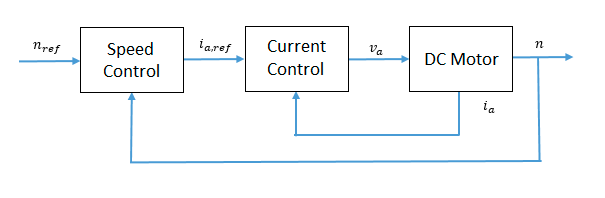
\includegraphics[width = \textwidth]{./pictures/dcmotorcontrol.png}
    \caption{DC motor control scheme}
    \label{fig:dcmotorcontrol}
\end{figure}

The scope of this thesis is to apply to hierarchical reinforcement learning the approach of control theory to  hierarchical control schemes, with small differences that are necessary in the context of learning. We have implemented a novel framework exploiting this approach, and thus fill up a gap between control theory and machine learning, based on one side on reinforcement learning and on the other side on optimal control. Exploiting the idea of cascaded blocks and inner/outer loops, our framework aims to make the hierarchy design for reinforcement learning intuitive. In the simplest form, the high level agent (outer loop controller) learns to drive the low level agent (inner loop controller) to the estimated goal point, whereas the low level agent adjusts its parameters to follow the reference given. This basic idea can be evolved further to adapt to more layers or to more complex topologies like switching between agents according to state as in hybrid systems.

When a problem with a continuous state and action space is considered, it may become impractical or non-satisfactory to employ value function based algorithms. On the other hand, policy search algorithms suffer from slow convergence.  In Hierarchical Policy Gradient Algorithms~\cite{GhavamzadehHierarchicalPG}, a possible solution to this conflict is presented benefiting the power of hierarchical structure to accelerate learning in policy gradient. 
We designed a simpler method to approach the same problem with a more compact representation exploiting our control theoretic framework.  

Corresponding field of reinforcement learning in control theory is optimal control. The similarity between the two fields becomes more evident once we rephrase the problem addressed by RL in terms of control theory. RL is inspired by behaviorist psychology, concerned with how agents should select actions in an environment, or, in other words, how they should adjust their policy in order to maximize the cumulative (discounted) reward ($\mathcal{J}$). The notion of cumulative reward translates to the negative of the cost function in optimal control ($\mathcal{C}=-\mathcal{J}$). The policy is the control law and the agent of RL is indeed the controller. Objective of RL written in these terms gives the goal of optimal control: to find a control law that minimizes the cost function. However, optimal control becomes weak when the model has strong nonlinearities and is analytically intractable or when approximations are not convenient. In contrast, reinforcement learning makes decisions interacting with its environment directly. Thus, the main difference between optimal control and reinforcement learning is the information used to build the model. In the RL approach, we do not attempt to analyze the dynamics of the environment to obtain a model or model parameters, but operate directly on measured data and feedback (rewards) from interaction with the environment. However, it is easy to spot analogies between the RL approach and optimal control. For instance the reward function selected can be the negative of the well known quadratic cost of the LQR, which describes a performance objective and punishes the control effort.

The system to be controlled can have a very complex structure and in some cases building a model can be impractical or not possible analytically. In control theory, an option to face the issue is to adapt the controller while interacting on the environment. An adaptive controller is composed of two subsystems: control unit and the tuning unit. Tuning unit is responsible to tune the parameters of the control unit which applies the control action to the environment, see~\ref{fig:adaptivecontrol}.
Referring to this structure, the counterpart of the tuning unit in RL is the learning algorithm and of the control unit is the policy itself.  However, even the adaptive control (or, to be more accurate, the controller that has been designed according to adaptive logic) assumes the knowledge of the environment’s description to a certain extent, at least in the form of a family of models that best describes it. In addition, adaptive control is mainly applied to the tracking and regularization type of problems rather than to optimal control ones. These form the fundamental contrasts between classical adaptive control and our approach. An exhaustive discussion of viewing reinforcement learning as adaptive optimal control is presented in~\cite{Sutton1991ReinforcementLI}.
\begin{figure}[t]
      \centering
	  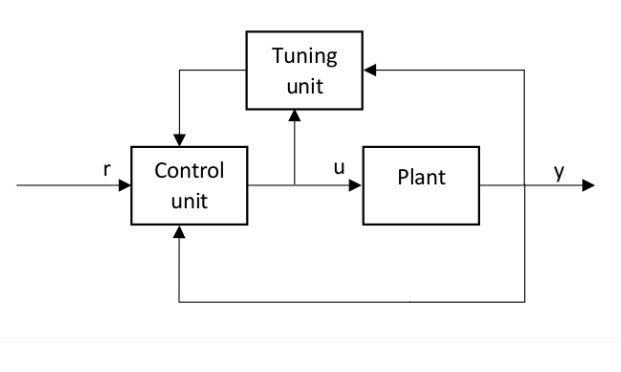
\includegraphics[width = 0.8\textwidth]{./pictures/adaptivecontrol.png}
      \caption{Adaptive control with two subsystems}
      \label{fig:adaptivecontrol}
\end{figure}

This thesis is organized as follows. 
In the second chapter, the state of the art is presented. Subsections include the titles Hierarchical Reinforcement Learning, Policy Search, Hierarchical Policy Gradient Algorithms.
In the third chapter the proposed method is described in detail. Implementation details are introduced in chapter four.
In the fifth chapter experimental setups for the proposed method are illustrated and results are discussed.
In the conclusion, the scope of the work and the evaluations are summarized and suggestions for future work are given.

\chapter{State of the Art}
\label{stateoftheart}
\thispagestyle{empty}

\begin{quotation}
{\footnotesize
\noindent{\emph{``Morty: I just I didn't get a lot of sleep last night. Maybe my dreams were just too loud or something.\\
Summer: Or maybe you were out all night again with Grandpa Rick. \\
Jerry: What? \\
Beth: Dad? \\
Rick: What, so everyone's supposed to sleep every single night now? You realize that nighttime makes up half of all time?''}}
\begin{flushright}
Rick and Morty (Season 1, Episode 1)
\end{flushright}
}
\end{quotation}


\vspace{0.5cm}

Many real-world problems are inherently hierarchically structured, meaning that it is possible look at a complicated challenge as a sequence of its more manageable components. As humans, we  tend to learn new tasks by breaking them up into easier ones and ordering them. A very simple real world example can be having a cup of coffee. The subtasks for this goal would be pouring the coffee, adding sugar, adding milk, and stirring. 

Artificial intelligence researchers benefited of this structure to afford clarity, concision and implementation hided in large scale tasks, using various ways of abstraction. Macros or macro operators form the fundamentals of the hierarchical notion in AI research. They can be used to group a whole series of actions into one and can be called as one primitive action. In addition, in the definition of a macro another macro can be defined. 

\section{Hierarchy in control systems}
\begin{figure}[t]
      \centering
      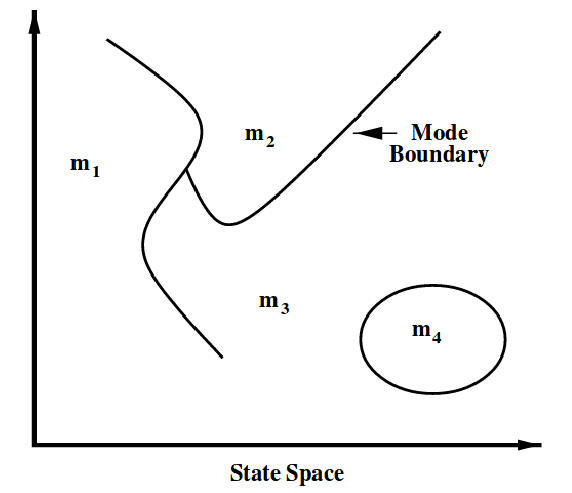
\includegraphics[width = 0.5\textwidth]{./pictures/modeswitching.png}
      \caption{Mode switching control}
      \label{fig:modeswitching} 
\end{figure}

In control theory, abstraction plays an important role. One way to implement the abstraction and hierarchy is to use hybrid systems. Hybrid systems are dynamical systems that exhibit both continuous and discrete dynamic behavior. When a control system is designed exploiting the hybrid formalism, typically, discrete controllers are in the higher levels of the hierarchy. This part is analogous to macros in AI research. In control theory, discrete action with respect to the state information is applied, and this action remains effective for an extended time. That is, discrete action changes the dynamics of the underlying controllers that act with continuous dynamics.

In AI terms a macro is called according to the state and it stays active until it terminates. Hybrid systems are a compromise between centralized and decentralized control schemes. In the centralized control scheme, the control signal is computed with the information from the entire system and then it is distributed to all the actuators. Despite its obvious advantages, such as having the possibility of global optimization, it is not practical as it requires high computational resources and the design tends to get tedious in large scale problems. In a completely decentralized control scheme, local controllers undertake the computation of commands for the subsystem actuators having limited information from the plant. Unlike the prior, they are easy to design. However, in cases of strong couplings between subsystems and/or where the closed-loop performance is crucial, this scheme is not adequate. When a decentralized solution cannot be accepted and a completely centralized solution is too expensive, a compromised scheme with some form of multilevel hierarchy is convenient. In the resulting systems, lower level deals with the local aspects of the performance whereas the higher level is responsible for the global criteria. In such hierarchy, the two levels possibly need different models of the plant. Local controllers need more detailed information on the dynamics of the part they act on and often they work with continuous models while for the higher level such details are impractical to handle. Thus, the typical choices for the higher level are discrete models. 

Mode switching controllers are a class of hybrid systems, where the control law depends on the location in state space, as in Figure~\ref{fig:modeswitching}. In other words, the higher level controller in the hierarchy switches between low level controllers according to the observation of the state. Mode switching controllers are commonly used in many control applications in order to allow relatively simple controllers to be used in different operating regimes, such as aircraft climbing steeply vs. cruising at constant elevation.
In~\cite{Grudic2000LocalizingSI}, the agent’s policy is designed as a deterministic mode switching controller and a new type of reinforcement learning called Boundary  Localized  Reinforcement Learning (BLRL) is proposed.

\section{Hierarchy in Reinforcement Learning}

Boundary  Localized  Reinforcement Learning (BLRL) is one of the many ways of defining a policy for a subset of a state in reinforcement learning. Examples of other forms of partial policies can be given as temporally-extended actions, options~\cite{Sutton1999BetweenMA}, skills~\cite{Thrun1994FindingSI} and behaviors~\cite{Brooksbehaviors, Huber1997AFC}. The idea of partial policies with well defined termination conditions is one of the key methods of temporal abstraction introduced to reinforcement learning to improve the scalability and enhance the performance. 

The nature of Markov decision processes (MDP), the models on which RL is based, does not involve actions that persist for an amount of time or, simply, temporally extended actions. In the classical MDP framework, an agent perceives the state of its environment at some discrete time t, takes an action accordingly, and, at the next time step t+1, gets from the environment a reward and the information about the next state s'. Moreover, the environment dynamics can be expressed with a transition function, which returns the probability of passing to state s’ given the current state s and the action a. Extension of the idea of higher level actions that contain lower level actions, which may or may not be the conventional one step actions, results in another type of decision process: semi-Markov decision process (SMDP). For SMDPs, the waiting time in state s upon the execution of action a is a variable and it represents relevant information. It corresponds to the execution time of a high-level action and depends on the policies and the termination conditions of all the lower-level ones. An SMDP consists of a set of states, a set of actions, an expected cumulative discounted reward for each state-action pair and a well-defined joint distribution of the next state and transit time. All three methods for introducing temporal extensions to actions that will be presented in this section, to explore the interaction between MDPs and SMDPs.

\subsection{Options}

An option is a temporally extended action with well defined policy. The term "option" is a generalization of primitive actions to adapt to the concept of temporal extension in SMDPs. In other words, an MDP  which has options instead of primitive actions is an SMDP. Figure~\ref{fig:options} from~\cite{Sutton1999BetweenMA} illustrates this definition. As mentioned above, the state trajectory of an MDP consists of small, discrete-time transitions, whereas that of an SMDP covers larger, continuous time transitions. Options enable an MDP trajectory to be analyzed in either way.
\begin{figure}[t]
      \centering
      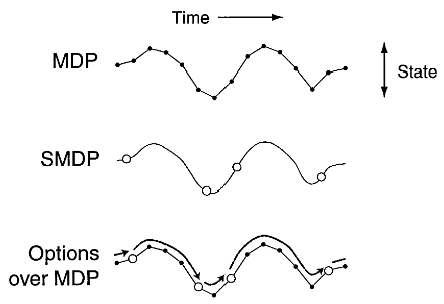
\includegraphics[width = 0.6\textwidth]{./pictures/options.png}
      \caption{Options over MDPs}
      \label{fig:options} 
\end{figure}
The main reason for the construction of options is to express temporally-extended actions in reinforcement learning and thus potentially increase the speed of learning in large-scale problems, particularly at the initial steps. Options can also assist the transfer of learning information between different tasks. For instance the option grab-the-door-knob whose policy is learned in open-the-door task might as well be used in close-the-door task. Though this advantage is highly dependent on the design of the options. This framework also facilitates adding prior knowledge to design. The designer of an RL system typically uses prior knowledge about the task to add a specific set of options to the set of available primitive actions.
An option has three components: a policy $\pi : \mathcal{S}^+\times\mathcal{A} \rightarrow \left[0,1\right]$, a termination condition $\beta: \mathcal{S} \rightarrow \left[0,1\right]$ and an initiation set $I \in \mathcal{S}$. An option is available only in the states that are contained in its initiation set. An option can be selected according to the policy over the options. If an option is selected, the policy of that option is followed until the option is terminated. The probability of an option to terminate in state s is given by $\beta(s)$. If the option does terminate, the agent gets to choose either a primitive action or another option that is available at the termination state of the previous one. Indeed, a primitive action can be considered as an option, called one-step option with $I=\{s: a \in \mathcal{A}_s\}$ and $\beta(s) = 1$ for all $s$. Each option can select another option, and so on, until one-step options are selected that correspond to the actions of the core MDP which leads to a hierarchical structure

\subsection{Hierarchy of Abstract Machines}

A machine is a partial policy represented by a Finite State Automaton. A Hierarchy of Abstract Machines (HAM)~\cite{Parr1997ReinforcementLW} is formed by the start of the execution of an initial machine and the termination of all the machines reachable from the initial one. Machines for HAMs are defined like programs that execute based on their own states, which can be of 4 types: \textit{action, call, choice} and \textit{stop}. In the \textit{action} states an action executes in the MDP. \textit{Call} sates, instead, start the execution of another machine. In \textit{choice} states, the next state of the machine is selected stochastically. \textit{Stop} halts the machine and returns the control to the previous call state. Apart from the set of states, a transition function and a start function which determines the initial state of the machine are needed in order to specify a machine. The transition function of a machine is defined as a stochastic function that depends on the current machine state and some features of the environment state and it determines the next state of the machine after an \textit{action} or a \textit{call} state. 

The interaction of a HAM $\mathcal{H}$ with an MDP $\mathcal{M}$ yields an induced MDP $\mathcal{H}\circ\mathcal{M}$. $\mathcal{H}\circ\mathcal{M}$ is indeed an MDP itself, with state set $\mathcal{S} = \mathcal{S}_M \times \mathcal{S}_H$, where $\mathcal{S}_M$ is the set of states of $\mathcal{M}$ and $\mathcal{S}_H$ is the set of states of $\mathcal{H}$. It is important to note that when we try to determine the optimal policy of $\mathcal{H}\circ\mathcal{M}$, the only relevant points are the \textit{choice} points. This is because, when $\mathcal{H}$ is in a state that is not a \textit{choice} state, only one action is allowed. These states can be eliminated to produce an SMDP called $\mathit{reduce}(\mathcal{H}\circ\mathcal{M})$. The optimal policy for $\mathcal{H}\circ\mathcal{M}$ will be the same as that of this SMDP, which, in turn, may increase the policy iteration speed. The above-mentioned property is particularly useful for RL. HAM constraints can reduce significantly the exploration effort by reducing the state-space in which the agent operates.

Options expand the repertoire of actions by defining the conventional primitive actions as a special form of options called one-step options, whereas HAMs are designed to constrain the set of allowed actions. For instance, in a case where an agent can choose up, down, right and left as actions, a machine may dictate “repeatedly choose right or down”. Such a command would erase the policies that choose  going up or left, which in return would simplify the MDP.

\subsection{MAX-Q Value Function Decomposition}
Another approach to HRL is the MAX-Q value function decomposition, developed in~\cite{Dietterich2000HierarchicalRL}. MAX-Q decomposes the value function of the main MDP into an additive combination of the value functions of the sub-MDPs.

To do so, MAX-Q takes an MDP $\mathcal{M}$ and decomposes it into a finite set of subtasks ${\mathcal{M}_0, \mathcal{M}_1, \mathcal{M}_2,\dotsc,\mathcal{M}_n}$. Here $\mathcal{M}_0$ refers to the root subtask. Once the root subtask is achieved the task itself is achieved. A subtask is formalized by a tuple $\langle \mathcal{T}_i, \mathcal{A}_i, \tilde{\mathcal{R}}^{i}\rangle$ where $\mathcal{A}_i$ is a set of admissible actions to achieve the subtask,$\mathcal{T}_i$ is a termination predicate that partitions the MDP states $\mathcal{S}$ into a set of active states $\mathcal{S}_i$ and a set of terminal states $\mathcal{A}_i$. A subtask can execute only in the states $s\in\mathcal{S}_i$ and once $\mathcal{M}$ goes into one of the states in $\mathcal{T}_i$, the subtask terminates. $\tilde{\mathcal{R}}^{i}$ is a deterministic pseudo-reward for each transition to a terminal state. By definition, $\mathcal{R}^{*i}$ is zero anywhere outside the terminal states. If the terminal state is the goal state, typically the pseudo-reward is zero again and for other terminal states it is negative. Each primitive action is a special case of subtask, as it was with options. $\mathcal{T}_i$ of a primitive action is that it terminates directly after the execution, $\tilde{\mathcal{R}}^{i}$ is uniformly zero and $\mathcal{A}_i$ contains a. For each subtask $\mathcal{M}_i$, a policy $\pi_i$ is defined. The hierarchical policy for the root task $\mathcal{M}_0$ is $\pi = \left\{\pi_0,\dotsc, \pi_n\right\}$. MAX-Q executes the hierarchical policy as the ordinary programming languages executes subroutines, using a stack discipline. That is, it explicitly defines a pushdown stack. Let us denote the contents of this stack at time t as $\mathcal{K}_t$. Once a subtask is active, its name and parameters are pushed up in the stack and once it terminates it is aborted from the stack together with everything that was above. 

Unlike the other two approaches, in this algorithm, the flow of information is from lower-level subtasks to higher-level subtasks only, and not vice versa. Due to this unidirectional flow of information, the decisions taken at a lower level will be independent of the higher-level goal to be achieved. It is easy to see that due to this additional restriction, the policies produced by this approach may not be hierarchically optimal but \textit{recursively optimal}. Recursive optimality is that the policy at each level is optimal assuming that policies of all lower levels are fixed. In general, a recursively optimal policy may not be hierarchically optimal and vice versa. A hierarchically optimal policy will always be at least as good as a recursively optimal one.

The idea of hierarchical policy is familiar from the discussion about the options. The policy over options, corresponds to that of the subtask in MAX-Q. In addition to that, the termination condition beta of the options framework translates to the termination predicate in MAX-Q. In this case, $\beta$ can only take the values  0 or 1 instead of a continuous interval between 0 and 1.

\section{Policy Search Methods}
Reinforcement learning in robotics is challenging, mainly due to the continuous action and state spaces. One technique to address this problem is discretization. However, particularly when considering actions with high dimensionality when a fine control action is needed, this approach becomes impractical. Most value-based reinforcement learning methods need to work on discrete actions, as they  estimate a value for state-action pairs and use the estimated values to build the policy: to produce a policy they need to search the action with the best value at each state, that can become impractical, unless the action set is discrete. 

An alternative to value-based methods is Policy search (PS).
PS methods start with a parameterized policy and try to find the parameters trough evaluating trajectories until a locally optimal solution is found. In robotics tasks, it is relatively simple to describe a family of suitable policies. Moreover, starting with a parameterized policy gives the opportunity to encode prior knowledge. Continuous action spaces are not an issue for PS, as the action is produced by the policy parametrization and no maximization of the action-value function is needed. For this reasons PS methods are frequently used in robotics. 

However, unlike value-based approaches, policy search might not converge to the global optima. In addition, they tend to converge slower than the value-based methods.

To take advantage from both PS and value-based approaches, Actor-critic algorithms where developed. Figure~\ref{fig:pstovaluebased} depicts these algorithms on the gray scale between purely value-based and purely policy search-based methods

\begin{figure}[t]
	\centering 		
    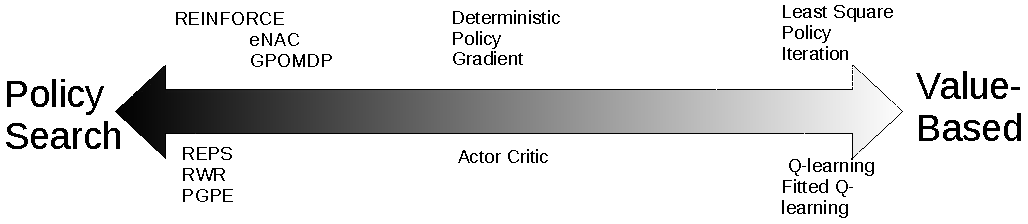
\includegraphics[width=\textwidth]{./pictures/greyscale.pdf}
    \caption[policy search, actor critic and value-based]{algorithms on a gray scale from direct policy search to value-based. Actor critic algorithm are in the middle.}
    \label{fig:pstovaluebased} 
\end{figure}


There are two ways of approaching PS: model-based and model-free. Model-based policy search addresses this problem by first learning a simulator of the robot’s dynamics from data. Subsequently, the simulator generates trajectories that are used for policy learning. It is interesting to note here that the differences between the adaptive control and the model-based policy search are indeed subtle. They both start with a class of models and predict a forward-model. When the interaction with the real robotic environment is difficult, due to safety or time constraints, model-based approaches are a preferable solution.

Model-free PS methods update the policy directly based on sampled trajectories and the obtained immediate rewards for the trajectories. Model-free PS methods try to update the parameters such that trajectories with higher rewards become more likely when following the new policy. Since learning a policy is often easier than learning an accurate forward model, the model-free approach is more used. 

The policy updates in both model-free and model-based policy search are based on either policy gradients (PG), expectation–maximization (EM) based updates, or information-theoretic insights (Inf.Th.). 

\subsection{Policy gradient}
With this method, parameters are updated with a gradient ascent so as to maximize the expected return, $\mathcal{J}_\theta$. The direction of the update is determined by the gradient $\nabla_\theta\mathcal{J}_\theta$. There are several ways to estimate this gradient. The simplest one of them is the finite difference method. The basic idea behind this method is to slightly perturb the parameters, $\delta\theta$, and examine the change in the reward, $\delta R$. The second method uses the likelihood-ratio approach: $\Delta p_\theta(y)=p_\theta(y)\Delta\log p_\theta(y)$. Likelihood ratio methods can be step-based or episode-based. Examples of step-based likelihood ratio methods are REINFORCE~\cite{Williams1992SimpleSG}, Gradient Partially Observable MDP (GPOMDP)~\cite{Baxter1999DirectGR, Bartlett2001InfiniteHorizonPE}. In REINFORCE and GPOMDP  algorithms the exploration is step-based, i.e., perturbation is applied to the actions at every time-step. Instead, Policy Gradient with Parameter Exploration Algorithm (PGPE)~\cite{Sehnke2008PolicyGW}, the exploration is done over the parameters, i.e., the perturbation is applied to the parameters at the beginning of the episode. The third method is based on the natural gradient. The key concept behind the natural gradient is to measure the distance between the distributions using the Kullback–Leibler divergence (KL) instead of using the euclidean distance between distribution parameters, to achieve a stable learning behavior. To achieve this goal natural gradient uses Fisher information matrix as metric. In this way, the gradient computed is invariant to the re-parametrization of the same policy, making the natural gradient also invariant to scale changes of the parameters. The computed gradient is rotated less than 90 degrees, therefore the same convergence properties of the vanilla gradient applies. Episodic Natural Actor Critic (eNAC)~\cite{Peters:2008:NA:1352927.1352986} is one of the algorithms that exploit this idea. 

\subsection{Expectation-Maximization (EM)}

The EM-based approach aims at making actions with high future reward more likely. EM formulates the policy search as an inference problem. The trajectories $\tau$ are the latent variables in the model and the observed value is the reward event. Then the classical EM algorithm is used to infer the new policy. Unlike the PG methods, since for most of the used policies there is a closed-loop solution, there is no need to determine a learning rate, which is a tricky task as it may lead to slow convergence or unstable policies. On the other hand, EM neglects the influence of the policy update on the trajectory distribution which can cause another problem: large jumps in the policy. It changes the behavior abruptly and there is a possibility that this new behavior may be extremely far from the optimal one, even damage the robot. Policy learning by Weighting Exploration with the Returns (PoWER)~\cite{Kober2008PolicySF} and Reward-Weighted Regression (RWR)~\cite{Peters2007ApplyingTE} are among the algorithms using this approach. PoWER uses episode-based exploration strategies with step-based evaluation strategies. PoWER is similar to episodic RWR but it has a more structured exploration strategy.

\subsection{Information Theoretic Approach (Inf. Th.)}
Information theoretic insight is exploited in Relative Entropy Policy Search (REPS)~\cite{Daniel2012HierarchicalRE, Peters2010RelativeEP}. It combines the advantages of two approaches described above. Instead of following the gradient, REPS formulates the policy update as an optimization problem. It tries to find the policy parameters that maximizes J while keeping bounded the KL w.r.t. the previous parameters. 

Using maximum likelihood estimates for the parameter updates is also beneficial for learning multiple solutions, as we can represent them with a mixture model. REPS can be extended to learning multiple solutions by reformulating the problem as a latent variable estimation problem, where the high level options are latent variables. The resulting algorithm is the Hierarchical Relative Entropy Policy Search (HiREPS)~\cite{Daniel2012HierarchicalRE} algorithm. 


\section{Hierarchical Policy Gradient Algorithm}

As discussed above, policy gradient algorithms are convenient for complex robotics tasks with high dimensions and continuous action spaces. However, they tend to suffer from slow convergence due to large variance of their gradient estimators. Hierarchical reinforcement learning methods gained the interest of researchers as a means to speed up learning in large domains. \cite{GhavamzadehHierarchicalPG} combines the advantages of these two and proposes hierarchical policy gradient algorithms (HPG). 

HPG objective is to maximize the weighted reward to go similar to~\cite{Marbach1998SimulationB} or~\cite{Bartlett2001InfiniteHorizonPE}. As the flat policy gradient algorithm, HPG searches for a policy in a set that is typically smaller than the set of all possible policies as it is parameterized and converges to local optimal policy rather than the global.  

In order to perform this approach, similarly to MAX-Q, the overall MDP $\mathcal{M}$ is divided into a finite set of subtasks. That is,${\mathcal{M}_0, \mathcal{M}_1, \mathcal{M}_2,\dotsc,\mathcal{M}_n}$ where $\mathcal{M}_0$ is the root task. The state space is divided into initiation and termination state sets for these subtasks and each subtask $\mathcal{M}_i$ that is not a primitive action has a policy $\pi_i$. The hierarchical policy is executed using a stack discipline. \cite{GhavamzadehHierarchicalPG} makes the assumption that the root task is episodic and also models the subtasks as an episodic problem. That is, all terminal states transit to an absorbing state $\ s^{*i}$ with probability 1 and reward 0.

\cite{GhavamzadehHierarchicalPG} suggests another method to speed up learning in HPG, called hierarchical hybrid algorithms in which some of the subtasks are formalized as value function-based reinforcement learning. These subtasks are in the higher levels where the action spaces are usually finite and the state relevant dimensions are fewer.  

Despite the obvious advantages, these algorithms are highly task-specific. That is, they are failing to build up a general framework for hierarchical policy gradient. Indeed the implementation of this algorithm for the ship steering task described in~\cite{GhavamzadehHierarchicalPG} is not trivial. It includes various shifts between different state-action spaces and intricate external reward definitions. Our approach aims to address these issues by implementing a framework that makes the hierarchy design for reinforcement learning more intuitive. 


\chapter{Proposed Method}
\label{proposed}
\thispagestyle{empty}

\begin{quotation}
{\footnotesize
\noindent{\emph{``Summer: A city of Grandpas? \\
Morty: It's the Citadel of Ricks. All the different Ricks from all the different realities got together to hide here from the government. \\
Summer: But if every Rick hates the government, why would they hate Grandpa? \\
Morty: Because Ricks hate themselves the most. And our Rick is the most himself.''}}
\begin{flushright}
Rick and Morty (Season 3, Episode 1)
\end{flushright}
}
\end{quotation}



\vspace{0.5cm}

In control theory, hierarchical architectures, where several layers of control interact, are extensively used. A very simple example is the cascaded control structure designed for a DC Motor where the outer loop (high level, slower) ensures that the actual speed is always equal to reference speed. In order to achieve its goal the outer loop outputs a reference torque/current which is received by the inner loop (low level, faster) that controls the torque via armature current and keeps the current in a safe limit. 

The design tool of control theory to approach hierarchical schemes is the block diagram. It gives the intuition of layered loops and cascaded structures. Block diagrams are much in use in control theory since they are often more convenient devices to analyze or design a system than the transfer function of the overall system. They are basically a composition of modular subsystems. These subsystems are represented as blocks that include the transfer function of the corresponding subsystem. The interconnections among subsystems are represented with directed lines illustrating the signal flow. We introduce these objects to hierarchical reinforcement learning with small differences that are necessary in the context of learning. The goal is to obtain a generic framework for the design of the hierarchy in reinforcement learning. This framework is a computational graph that contains various types of blocks referring to subsystems. Unlike the block diagram of control theory, in our approach blocks and the interconnections are of various nature.

In our scheme one cycle of the computational graph corresponds to a step in the environment. At each step, environment observation is retrieved in the form of a reward and a state data. A state can be absorbing or not. If it is, then the graph is at the last cycle of the current episode. Otherwise, an action, taken from the last block in the graph, is applied and the environment state is observed once again and so on. Data flow in the graph through connections between blocks. There are three types of connections: input, reward, and alarm connections. Input connections correspond to the connections in the conventional block diagram. They transport input and output data between blocks. We call the input signal of a block as \textit{state} and the output as \textit{action}. It should be remarked that the terms state and action here do not refer to the content of the data carried but to the manner in which the receiving block perceives them. For instance, reward data of the environment can be observed as the state by some blocks. Hence, the connection that carries the reward would be the input connection.

RL agent aims to approximate an optimal behavioral strategy while interacting with its environment. It evaluates its behavioral strategy based on an objective function $(\mathcal{J})$ that is computed with rewards. These rewards can be extrinsic or intrinsic. Extrinsic rewards are in the formalization of the environment. They are retrieved through observation. Intrinsic rewards can be constructed by the designer using the state information. In optimal control, typically, the performance indicator is the cost function $(\mathcal{C = -J})$ and the optimal control goal is to find a control law that minimizes the cost function. In optimal control, the cost function is optimized at design time. That is, unlike the RL agent, during its operation, the controller does not need a metric to evaluate and update its behavior. This contrast reflects in our framework into another type of connection that carries only the reward information. An explicit reward connection definition is needed. Reward connection implies that the data carried will be used as a performance metric and not as an input to the block. 

In hierarchical approaches to RL, typically, high level agents do not take actions at each step. To enforce this structure in our framework, blocks that are in the higher levels of the hierarchy are not activated in some cycles. Their output remains unchanged for those time steps. Once the lower level blocks complete their episode they activate the upper level ones by sending a signal trough alarm connections. 

\begin{figure}[t]
      \centering
      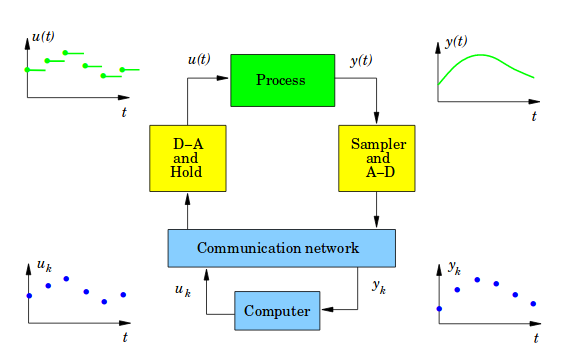
\includegraphics[width = \textwidth]{./pictures/digitalcontrol.png}
      \caption[Digital control system]{Schematic of a digital control system}
      \label{fig:digitalcontrol}
\end{figure}

In this scheme, alarms are analogous to events in event-based control systems. Event-based control systems are digital control methods. Figure~\ref{fig:digitalcontrol} shows a typical architecture for a digital controller. The process is a continuous-time physical system to be controlled. The input and the output of the process are continuous-time signals. Thus, the output needs to be converted and quantized in time before being sent to the control algorithm. This process is called \textit{sampling}. There are two ways of designing digital controllers: periodic and event-based trigger. The traditional way to design digital control systems is to sample the signals equidistant in time, that is, periodically~\cite{aastrom1997computer}, using a clock signal.  

Event based sampling is an alternative to periodic sampling. Signals are sampled only when significant events occur. This way, control signal is applied only when it is required, so as to better cope with various constraints or bottlenecks in the system. A block diagram of a system with event based control is shown in \ref{fig:eventbased}. 

\begin{figure}[t]
	\centering
    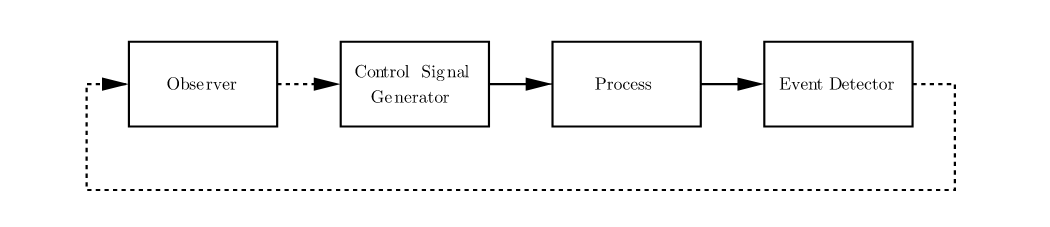
\includegraphics[width=\textwidth]{./pictures/eventbased.png}
    \caption[event-based control]{Block diagram of a system with event-based control. Solid lines denotes continuous signal transmission and the dashed lines denotes event based signal transmission}
    \label{fig:eventbased}
\end{figure}
  
The system consists of the process, an event detector, an observer, and a control signal generator. The event detector generates a signal when an event occurs, typically when a signal passes a level, possibly with different events for up-and down-crossings. The observer updates the estimates when an event occurs and passes information to the control signal generator which generates the input signal to the process. The observer and the control signal generator run open loop between the events. The dashed lines of Figure~\ref{fig:eventbased} correspond to the alarm connections in our framework. In HRL approaches, typically a lower-level algorithm returns to the higher-level one once it has completed its subtask. It can be due to an absorbing state terminating either with success or failure, or simply a horizon reach. The event of event-based control thus corresponds to the end of a subtask of a low-level agent in HRL. 

In control theory, each block of the block diagram refers to a subsystem such as a plant, a controller or a sensor, and contains the corresponding transfer function or state-space equation matrices. Either way, it includes an expression of how the incoming signal is manipulated. \ref{fig:blockdiagramofcontrolth} depicts an example structure. Apart from the blocks and connections, there are circle shaped objects in the diagram which represent basic arithmetic operations applied to the incoming signals. 

\begin{figure}[t]
      \centering
      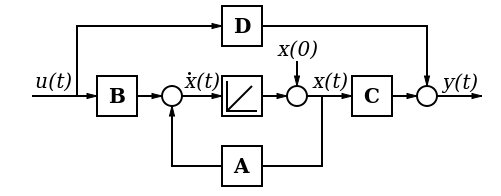
\includegraphics[width = 0.8\textwidth]{pictures/blockdiagramofcontrolth.png}
      \caption{Example of a conventional block diagram}
      \label{fig:blockdiagramofcontrolth}
\end{figure}

Blocks in our framework have subtle differences. The manner in which the signal is manipulated explicitly depends on the type of the block. The input-output relation of some of the blocks have a discrete-time dynamic behavior. They keep track of the state and store information. That is, they are stateful and their operation can be described with a discrete-time transfer function. \textit{function block} is the most similar kind to a conventional block of control theory. Its operation on the incoming signal is deterministic. In other words, it has a deterministic policy chosen by the designer of the system. Function block is an example to stateless blocks. A type of function block performs simple arithmetic operations on the incoming signals. They are named as \textit{basic operation blocks}. 

Control block is the learning part of the system. It is associated to a policy and a learning algorithm. It calls the policy to take an action and uses the learning algorithm to update the policy. This learning algorithm can be policy search-based (e.g. GPOMDP, PoWER) or value-based (e.g. Q-learning, SARSA($\lambda$)) and the policy can be a parameterized one (e.g. Gaussian) or a Q-value-based one (e.g. Boltzmann, $\epsilon$-greedy). Control blocks accumulate each trajectory sample in a dataset. Once the policy is to be updated, this dataset is passed to the learning algorithm. Similarly to the MDPs a sample $\left\langle s,a,r,s'\right\rangle$ consist of state, reward, action and next state data, being the input, the output and the reward of the block.
In a control block the state and reward data are manipulated separately. State data flow is used for computing the value of the blocks and action, i.e. running the system, whereas the reward data flow is the flow of the evaluation of the performance. Thus, control block needs reward connections to be isolated from the input connections.

Naturally, control blocks are the only blocks at the receiving ends of the reward connections as they are the only learning members. The other blocks may also take extrinsic reward data from the environment. However, they will not perceive it as a performance metric. Thus, they will receive the data through input connections instead of a reward connection.

If the control block is in a lower level of the hierarchy, it can signal the end of its episode to the higher level blocks. The end of an episode can be reached due to an absorbing state with failure or success or a horizon reach. The control block that is in the higher levels of the hierarchy does not take an action until it receives an alarm signal or an indicator of a last step of the environment.  

Apart from the end of an episode of a control block, custom events can be created to produce alarm signals. Event blocks are used with this objective. 
They have custom methods with binary results.

Since some of the control blocks are \textit{awake} only at certain times, some measures needs to be taken to protect the integrity of their dataset. Reward data coming from the environment must not be lost when the high level control is inactive. Reward accumulator block accumulates the input reward until the alarm is up. With the alarm, accumulated data is passed to the controller and the accumulator is emptied. Obviously, the alarm source that is connected to a high level controller needs to be the same as the one that is connected to the reward accumulator that passes its data to that controller. Since the reward accumulator stores information, it is an example of a stateful block.

Another example of a stateful block is the error accumulator. Error accumulator block accumulates the incoming error data and passes it at each step to a control block. When one of its alarms activates or the environment state is the last of the episode it resets the accumulator to zero. Integration in discrete time corresponds to accumulation. The control block that has an error accumulator as an input connection applies integral action. 
  
Placeholders operate as the representation layer of the environment. In the conventional block diagram, the model of the plant is a part of the block diagram. Typically, it receives control signal as an input and outputs the state data to the rest of the blocks. It contains the transfer function of the plant model. In our framework, the model itself is not a part of the diagram. This is primarily because we focus on model-free learning, thus we do not have a mathematical expression of how the environment reacts to inputs, nor its estimation. The only information we have comes from the step samples. The other reason is that blocks may need to observe different parts of the environment. For instance, a block may require only the reward to operate whereas the other one may need both the state and the reward. Such isolation of observation data is achieved with placeholders. At each cycle of the graph, state and the reward output of the environment are passed through the related placeholders, the state and reward placeholders. In addition, last action applied to the environment is also saved in a placeholder called last action placeholder. These blocks do not operate on or manipulate the data they receive. Instead, they function as a bridge or a network between the environment and the diagram. 

Selector blocks implement the mode switching behavior in our framework. They contain block lists and activate one list at each cycle. The selection is done according to the first input of the selector block. Once a list inside the selector block is activated all the other inputs to the selector block are passed to the first block of the selected list. The reward and alarm connections of the blocks inside the selector block are independent from the selector. That is, selector block does not have reward connections and its alarm connections are not passed to the blocks in the block lists. Selector block strengthens the flexibility of our framework for hierarchical schemes by allowing hybrid schemes to join the picture. Higher level controller applies an action depending on the state and this action activates an underlying behavior provided by the selected block list in the selector block.



\chapter{System Architecture}
\label{architecture}
\thispagestyle{empty}

\begin{quotation}
{\footnotesize
\noindent{\emph{``Morty: I mean, why would a Pop-Tart want to live inside a toaster, Rick? I mean, that would be like the scariest place for them to live. You know what I mean?\\
Rick: You're missing the point Morty. Why would he drive a smaller toaster with wheels? I mean, does your car look like a smaller version of your house? No. ''}}
\begin{flushright}
Rick and Morty (Season 1, Episode 4)
\end{flushright}
}
\end{quotation}



\vspace{0.5cm}

The framework implements three layers: hierarchical core, computational graph, and the blocks. The implementation details of these layers and of other utility functions are presented in this chapter. Figure \ref{fig:overall} illustrates the architecture of the system.

The framework exploits \texttt{mushroom}~\cite{mushroom}, a reinforcement learning library of AI\&R Lab of Politecnico di Milano, which provides learning algorithms, features, environments, policies, distributions and function approximators. Apart from the methods implemented, our framework adopts some of the design concepts of the \texttt{mushroom} library. Datasets are formed with the same structure, that is, every step is represented with a tuple containing state, action, reward, next state, and the absorbing and last step flags. In addition, the hierarchical core is indeed a hierarchical version of mushroom core. Our framework is implemented to be compatible with any flat reinforcement learning mushroom algorithm.

\section{Hierarchical Core}
Hierarchical core unit is developed as an interface between the diagram and Python. A computational graph is passed to the hierarchical core in the declaration. The hierarchical core contains the methods to run it with a requested amount of steps or episodes. In the beginning of each run the hierarchical core initiates the computational graph and at the end of the runs calls it to stop. The runs can be made for the hierarchical algorithm to learn or to evaluate its performance. During the learning runs, policies of blocks with a learning algorithm in the computational graph are updated. A flag is passed to the computational graph to signal the mode of the run. 

\begin{figure}[t!]
      \centering
      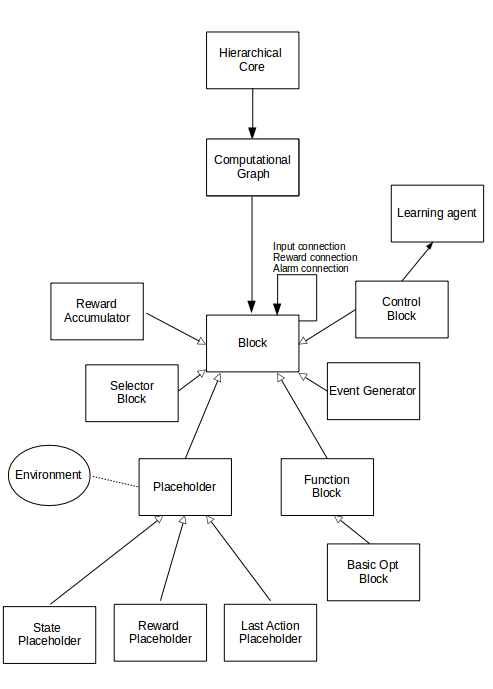
\includegraphics[width = \textwidth]{./pictures/overall_new.png}
      \caption{System architecture}
      \label{fig:overall}
\end{figure}

\section{Computational Graph}
Computational graph establishes the connection between the environment and the block diagram. In the declaration, it receives a list of blocks and a model. 

When the computational graph calls a block, it sends a request to that block to activate its functionality. To call a block, computational graph checks the input, reward and alarm connections of that block. The last outputs of the input connection blocks are passed in an input list. A block can have one reward connection at most. The last output of the reward connection block, if exists, is passed as a reward. The alarm output of the alarm connections are passed as alarms. If a block does not have an alarm connection, it should wake up at each state. Thus, a default alarm is passed in such cases. Finally, in order to indicate the blocks whether or not they should update their policy, a learn flag is passed.

Computational graph calls the blocks in the sorted list one by one until the cycle completes. Each cycle corresponds to a step of the environment. 
At the start of each episode, the computational graph takes the initial state of the environment, and all the blocks are called for a reset. The first primitive control action, that is the last output of the last block in the sorted block list, is stored in the last action placeholder. Computational graph starts each cycle by applying the primitive control action to the environment. Then, the computational graph observes the response of the environment in the form of a state and reward data. The state and reward data are passed to the corresponding placeholders. The state of the environment can be absorbing due to success or failure which results to terminate the episode. Another reason for a step to be the last of the current episode is that the environment horizon is reached. Two variables that signal the last and the absorbing states of the environment are passed to the blocks by the computational diagram when they are called.

In order to activate the blocks in the correct order, computational graph needs them to be sorted in accordance with their connections, using a topological sort algorithm. To achieve this, the block diagram is described as a directed graph where each node is a block and the edges are the connections between them. Placeholders are not considered during the construction of the graph. This is because, as described previously in chapter~\ref{proposed}, placeholders are not called as the other block objects. They are employed to pass the environment data to the rest of the graph. Thus, regardless of their connections, they ought to be the first ones in the list. In fact, placeholders do not need to have a connection as their input connection is the environment itself and the environment is not a part of the block diagram. Therefore, they are not declared as nodes and thus no edges are created between any other blocks and placeholders. Additionally, the blocks that are members of the block lists inside the selector blocks are not included in the block list passed to the computational graph. These blocks retrieve their inputs through the selector block. However, their reward connections are independent of the selector block. To maintain the integrity of the topological sort, while constructing the graph for sorting, connections of these blocks are represented as the connections to the selector block. 
This graph is sorted with a function already implemented in the \texttt{networkx} library. The sorted block list that the computational graph uses is a concatenated list of placeholders and the blocks sorted with the above-mentioned algorithm.
Computational graph calls the blocks also to initialize and to stop at the end of runs, when it is asked by the hierarchical core.

\section{Blocks}
In our framework, blocks are of various types reflecting the subsystem that they represent. Blocks superclass has a name, a last output, an alarm output, and lists for various types of connections that contain the connected blocks. Blocks have methods to add input, reward, or alarm connections to their lists. Computational graph calls the blocks. Blocks may or may not accept the call. A call is accepted only when the alarms of the called block are up or when it is the end of an episode for an environment. If the call is accepted, block updates its last output and its alarm output with a method implementation that depends on the type of the block. Blocks are asked to initialize by the computational graph at the beginning of each run. At the end of each episode of the environment they are reset. 

\subsection{Function Block}
A function block is declared with a name and a custom function. When the call from the computational graph is accepted, that is, at least one of the alarm connections returns true or the environment is at its last step, the last output of the function block is updated. This update is done passing the inputs of the function block as a parameter to the custom function. Reset method of the function block operates similarly, except in this case no conditions are defined to update the last output. When initialized, all outputs are set to \texttt{None}. Summation, sign, and squared norm operations are defined and named respectively as: \texttt{addBlock}, \texttt{signBlock}, and \texttt{squarednormBlock}. 

\subsection{Event Generator}
Event generator block implementation is similar to that of the function block. In the declaration, a custom function is passed. This function needs to have a boolean return since the event generator triggers the alarms which can be either up or down. Once the event generator accepts the call of the computational graph, it updates its alarm output with the custom function. When it is called to reset, it updates its alarm output regardless of the state of the connections and the environment. Its last output is always \texttt{None}. 

\subsection{Control Block}

Control block runs the policy/subtask for a period of time that is in general independent from that of the environment. This is because the episode of the subtask is different from that of the task. That is, subtasks have their own termination conditions and horizons.

Control block requires the designer to pass a learning algorithm, number of episodes or number of steps per fit, optionally a termination condition and callbacks during the declaration. It has its own dataset and the dataset is passed to the learning algorithm when the number of episodes or the number of steps per fit is reached and when the hierarchical core is executing a learning run.

Each sample of the dataset is a tuple that contains the state, action, reward, next state, and the absorbing and last step flags. Every time the call of the computational graph is accepted, control block takes a step. If it is the first step of its own episode, it resets. The class method reset calls the learning algorithm to start an episode and draw an action. The current inputs and the action drawn are saved as the first samples of the state and action respectively and the last output of the block is set to the action. In the later steps, the horizon and the termination condition is checked to see whether the current state is absorbing or the last of its episode for the control block. A sample is taken that contains the state, reward and the two flags that indicate the absorbing and last states of the block. Combined with the previous sample, it builds up a step tuple for the control block dataset. State and action data of the previous sample are the state and action of the step tuple and the state of the current sample is the next state. 

Once the step tuple is appended to the dataset, control block checks for the fit condition. If the fit condition is satisfied, i.e., if the number of episodes or the number of steps per fit is reached and the hierarchical core is executing a learning run, it passes the dataset to the learning algorithm to fit, clearing the dataset. The callbacks passed in the declaration will be called during the fit, with the dataset passed. 

If the state is not the last of its episode for the environment, an action is drawn and saved as the last output of the control block. An action must be drawn even when the control block reached its horizon or when its termination condition is satisfied. This is because in the framework, each cycle of the computational graph corresponds to a step in the environment and it is not possible to go back to the higher level controller during the cycle. Another cycle is needed to reset and start a new episode for the low level controller that has its episode finished. This makes our framework operate in a way slightly different from the other HRL approaches, such as MAXQ, that use a stack discipline.

The action taken is sampled for the next step tuple. Control block needs to signal the end of its episode to the higher level blocks in the hierarchy. Hence the alarm output is set to the value of the flag that indicates the last step of an episode.

When the computational graph asks for a control block to initialize, control block empties its dataset and sets its last output to \texttt{None} and the alarm output to \texttt{False}. When the learning or the evaluation run is over, control block calls the learning algorithm to stop.

\subsection{Placeholders}
Placeholders are the first blocks to be called in the cycle and serve as a presentation layer of the environment model. Placeholders have \textit{null} operation in their call, reset and initialize methods. Their last output is assigned by the computational graph using the samples from the environment and the last output of the last block in the ordered list.

\subsection{Selector Block}
The purpose of the selector block is to activate just a chain of blocks avoiding the other blocks to take actions and fit when they are not active. This way we can avert the accumulation of the dataset for the inactive blocks. To implement this behavior, selector block contains block lists ad activates just one list of blocks at each cycle. The selection is done according to the first input of the selector block. Once a list inside the selector block is selected, the rest of the inputs of the selector block are passed to the first block of the selected list. The operation of a selector block is similar to that of the computational graph from this perspective. It calls the blocks in that list one by one passing the inputs, rewards and alarms according to the connection lists of the corresponding blocks. However, selector block does not sort the blocks. Instead, it calls them in the provided order in the list. Selector block manages a boolean list named \texttt{first},s used as an indicator of whether or not the corresponding block list is being called for the first time after a reset or not. This information is necessary for the proper operation of blocks and to preserve the integrity of the dataset of the control blocks in the list. Initially, all flags are set to True. When the computational graph asks for a reset, selector block resets the blocks in the selected block list. It does not request the other block lists to reset as this operation includes taking an action, and selector block must avoid calls to blocks in inactive block lists. Then, the indicator of the selected block lists is set to False. If the selector block is calling the block list before having it reset, i.e. if the first flag for the selected block list is True, selector block resets the blocks in that list instead of calling them. 
At the beginning of each run, selector block asks all the blocks in the lists to initialize and sets the first flags to True. At the end of runs, all control blocks in the lists are stopped. 





\chapter{Experimental Results}
\label{experimental}
\thispagestyle{empty}

\begin{quotation}
{\footnotesize
\noindent{\emph{``Rick: Come on, flip the pickle, Morty. You're not gonna regret it. The payoff is huge.
(Morty hesitantly picks up the screwdriver and turns the pickle over. The pickle has Rick's face on it) I turned myself into a pickle, Morty! Boom! Big reveal: I'm a pickle. What do you think about that? I turned myself into a pickle! W-what are you just staring at me for, bro. I turned myself into a pickle, Morty! \\
Morty: And? \\
Rick: "And"? What more do you want tacked on to this? I turned myself into a pickle, and 9/11 was an inside job?\\
... \\
Morty: I-I'm just trying to figure out why you would do this. Why anyone would do this. \\
Rick: The reason anyone would do this is, if they could, which they can't, would be because they could, which they can't.''}}
\begin{flushright}
Rick and Morty (Season 3, Episode 3)
\end{flushright}
}
\end{quotation}

 


\section{Ship Steering Domain}
We chose ship steering task~\cite{Anderson:1990:CSC:104204.104226} to test the framework. Ship steering has complex low level dynamics due to its continuous state-action space and it is well suited for designing hierarchies. The task was initially studied as a control theory problem~\cite{shipsteeringACD}. Later, \cite{GhavamzadehHierarchicalPG} introduced the problem to machine learning literature and suggested Hierarchical Policy Gradient Algorithms as a solution. 
Ship steering domain is shown in Figure \ref{fig:shipsteeringdomainbig}.

\begin{figure}[t]
      \centering
      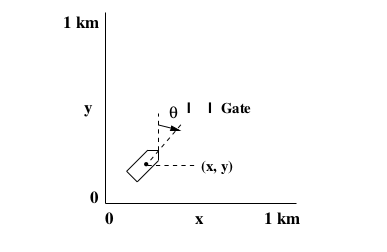
\includegraphics[width = 0.5\textwidth]{./pictures/shipbigenv.png}
      \caption{Ship steering domain}
      \label{fig:shipsteeringdomainbig}
\end{figure}
    
A ship starts at a randomly chosen position, orientation and turning rate and has to be maneuvered at a constant speed through a gate placed at a fixed position in minimum time. Since the ship speed is constant, minimum-time policy is equivalent to shortest-path policy. We consider the ship model given by a set of nonlinear difference equations~\ref{eqn:shipsteeringequation}.

\begin{equation}
\label{eqn:shipsteeringequation}
\begin{split}
     &x\left[t+1 \right] = x[t] + \Delta V \sin \theta \left[t\right]\\
     &y\left[t+1 \right] = y[t] + \Delta V \cos \theta \left[t\right]\\
     &\theta\left[t+1 \right] = \theta[t] + \Delta \dot{\theta} \left[t\right]\\
     &\dot{\theta} \left[t+1\right] =  \dot{\theta} \left[t\right] +\Delta (r\left[t\right] - \dot{\theta}\left[t\right])/T
\end{split}
\end{equation}
where $T = 5$ is the constant time needed to converge to the desired turning rate, $V = 3\frac{m}{s}$ is the constant speed of the ship, and $\Delta = 0.2 s$ is the sampling interval. The control interval is $0.6 s$ (three times the sampling interval).
There is a time lag between changes in the desired turning rate and the actual action, modeling the effects of a real ship’s inertia and the resistance of the water. The state variables are the coordinates ($x$, $y$), the orientation ($\theta$) and the actual turning rate of the ship ($\dot{\theta}$). The control signal is the desired turning rate of the ship ($r$). The state variables and the control signal are continuous within their range given in the table \ref{table:ranges}.

\begin{table}[t]
  \centering
  \begin{tabular}{c r r}
     \toprule
     Variable & Min & Max \\
     \midrule
     $x$ & 0 & 1000 \\ 
     $y$ & 0 & 1000 \\
     $\theta$ & $-\pi$ & $\pi$ \\
     $\dot{\theta}$ & $-\frac{\pi}{12}$ & $\frac{\pi}{12}$ \\
     $r$ & $-\frac{\pi}{12}$ & $\frac{\pi}{12}$ \\
     \bottomrule
  \end{tabular}
  \caption{State and action variable ranges}
  \label{table:ranges}
\end{table}

The ship steering problem is episodic. In each episode, the goal is to learn the sequence of control actions that steer the center of the ship through the gate in the minimum amount of time. To make sure the optimal policy is to find the shortest path, every step of an episode has a reward of -1. If the ship moves out of bound, the episode terminates and is considered as a failure. In this case, environment returns -100 as a reward. The sides of the gate are placed at coordinates (350,400) and (450,400). If the center of the ship passes through the gate, episode ends with a success and a reward 0 is received. 

The task is not simple for classical RL algorithms for several reasons~\cite{GhavamzadehHierarchicalPG}. First, since the ship cannot turn faster than $\frac{\pi}{12} \frac{rad}{s}$, all state variables change only by a small amount at each control interval. Thus, we need a high resolution discretization of the state space in order to accurately model state transitions, which requires a large number of parameters for the function approximator and makes the problem intractable. Second, there is a time lag between changes in the desired turning rate $r$ and the actual turning rate, ship’s position $x$, $y$ and orientation $\theta$, which requires the controller to deal with long delays. In addition, the reward is not much informative. 

Thus, we used a simplified version of the problem for the early experiments. The simplified ship steering domain is given in Figure~\ref{fig:shipsteeringdomain}. The domain boundaries are smaller, to shrink the state space. Ranges of the state and action variables are given in Table~\ref{table:rangessmall}. In this case, the gate is positioned in the upper right corner of the map at the coordinates (100,120) and (120,100). The ship starts at the origin of the state space, i.e., fixed at position (0, 0) with orientation 0 and no angular velocity.   
\begin{figure}[t]
      \centering
      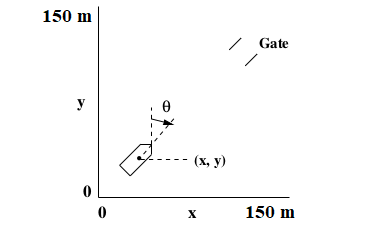
\includegraphics[width = 0.45\textwidth]{./pictures/shipsteeringdomain.png}
      \caption{Ship steering small domain}
      \label{fig:shipsteeringdomain}
\end{figure}

\begin{table}[t]
  \centering
  \begin{tabular}{c r r}
     \toprule
     Variable & Min & Max \\
     \midrule
     $x$ & 0 & 150 \\ 
     $y$ & 0 & 150 \\
     $\theta$ & $-\pi$ & $\pi$ \\
     $\dot{\theta}$ & $-\frac{\pi}{12}$ & $\frac{\pi}{12}$ \\
     $r$ & $-\frac{\pi}{12}$ & $\frac{\pi}{12}$ \\
     \bottomrule
  \end{tabular}
  \caption{State and action variable ranges for small environment}
  \label{table:rangessmall}
\end{table}

\section{Flat Policy Search Algorithms}
Experiments with flat PS algorithms are implemented for the small domain using \texttt{mushroom} library. The flat algorithms use a tiling with three dimensions to divide the state space $5 \times 5 \times 6$ tiles each. 100 experiments have been carried out for each flat algorithm. Every experiment lasted 25 epochs. In every epoch, the learning algorithm runs for 200 episodes. Then the evaluation run is carried out. The resulting dataset of the evaluation run is used to compute cumulative discounted rewards ($\mathcal{J}$) for each episode in the evaluation dataset and averaged for each epoch. With the same method, also the mean length of the episodes for each epoch is computed. These data are averaged for 100 experiments.

For the major part of the experiments, PG algorithms are implemented with an adaptive learning rate. Adaptive learning rate constrains the step of the learning algorithm with a given metric, instead of moving of a step proportional to the gradient. The step rule is given in Equation~\ref{eqn:adaptivelr}. Adaptive learning rate can be used to prevent jumps when the gradient magnitude is big. 

\begin{equation}
\label{eqn:adaptivelr}
    \begin{aligned}
    \Delta\theta=\argmax_{\Delta\vartheta}\Delta\vartheta^{t}\nabla_{\theta}J
    \\
    s.t.:\Delta\vartheta^{T}M\Delta\vartheta\leq\varepsilon
    \end{aligned}
\end{equation} 


GPOMDP, a step-based PG algorithm, has been implemented to learn the parameters of a multivariate Gaussian policy with diagonal standard deviation. The initial standard deviation ($\sigma)$ is set to $3\times10^{-2}$. The mean of the Gaussian is formulated with a linear function approximator with tiles. Learning parameter is adaptive with a value of $10^{-5}$. Policy is fit every 40 episodes during the learning run. Number of episodes of an evaluation run is also 40. 

RWR, REPS and PGPE algorithms work on a distribution of policy parameters and they can be used with deterministic policies. They have been implemented to learn the distribution of the mean $\mu$ of a deterministic policy. Mean is linearly parameterized with the tiles. The distribution is a Gaussian distribution with diagonal standard deviation. The initial mean $\mu$ is the null vector, and $4\times10^{-1}$ variance $\sigma^2$ for every dimension. All three algorithms are run for 200 episodes to learn at each epoch. Every 20 episodes, the distribution parameters are updated. The evaluation run lasts 20 episodes. The learning rate of PGPE is adaptive and the value is initially set to $1.5$. REPS and RWR do not require the learning rate to be specified as explained in Chapter~\ref{stateoftheart}. REPS is used with a max KL step $\epsilon = 1$, and RWR with a constant $\beta = 0.7$ for the exponential transformation. 

\section{Hierarchical Block Diagram Approach}

The ship steering control system consists fundamentally of two parts~\cite{shipsteeringACD}:
 
\begin{itemize}
   \item a ship autopilot which automatically manipulates the rudder to decrease the error between the reference heading angle and the actual heading angle, and
   \item an operator, either human or a machine, that closes up the control loop given the reference angles to follow a desired trajectory on the ocean.
\end{itemize}

The control theory approach to ship steering problem is preserved for the subtask definitions with our framework. The corresponding block diagram is given in Figure~\ref{fig:blockdiagramship}. 

\begin{figure}[t] 
      \centering
      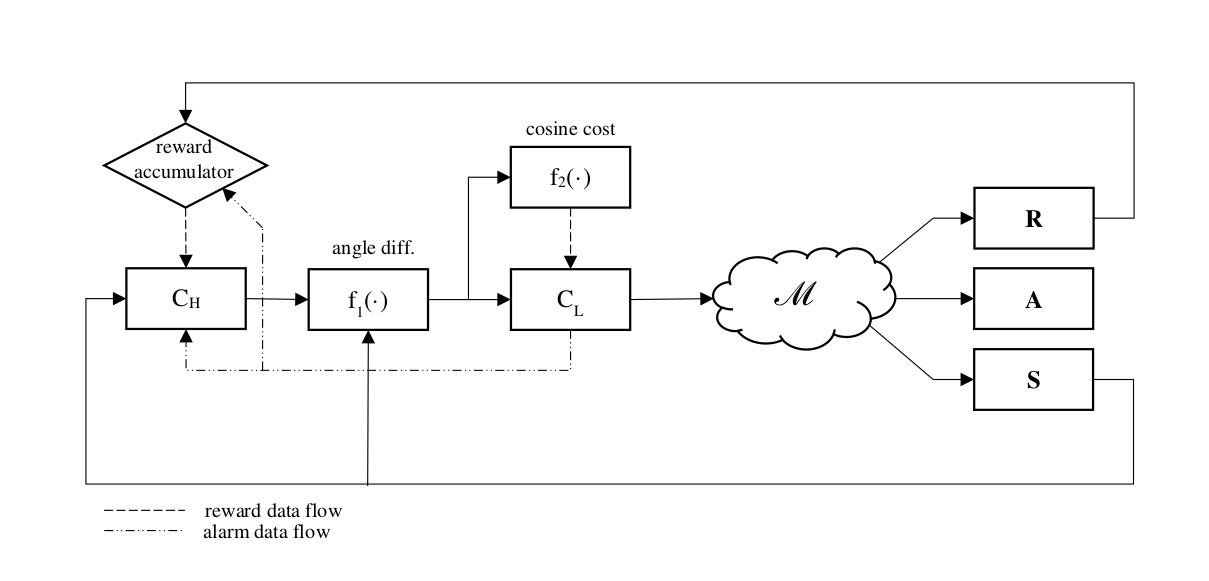
\includegraphics[width = \textwidth]{./pictures/blockdiagramshipsteering.png}
      \caption{HRL block diagram for ship steering task}
      \label{fig:blockdiagramship}
\end{figure} 

Low level controller learns to approximate the optimal policy to decrease the error between the reference angle and the actual angle.  High level controller learns to drive the low level by producing reference positions in the map that approximate the shortest paths to the gate. A function block in between the control blocks ($f_1( \cdot )$) computes the reference angle for the low level, given the reference position and the states. The performance metric of the high level control is the extrinsic reward, whereas the one of the low level is computed by another function block, $f_2( \cdot )$. $f_2( \cdot )$ returns the cosine of the angle difference computed by $f_1( \cdot )$. As the difference of the reference angle and the actual angle gets close to 0, the reward advances to 1 and as it grows, the reward decreases to -1. 

When the low level controller finishes its episode, it raises an alarm for the high level. In the following cycle, a new reference point is estimated for the level. The same alarm signal is passed to the reward accumulator of the high level controller with the motivations described in Chapter~\ref{proposed}. 

The high level controller uses the GPOMDP algorithm to learn a multivariate Gaussian policy with diagonal standard deviation. Its mean is initialized in the middle of the map, that is $(75, 75)$, for the small domain. The variance of both dimensions is $40$. The algorithm fits every 20 episodes with an adaptive learning rate of 10. Horizon is 100 steps for both controllers.

Low level control policy should steer the ship in the direction of the angle error. That is, if the reference angle is larger than the current angle, angular velocity output of the low level control should be positive and vice versa. Low level controller is first tested with a GPOMDP algorithm with a differentiable parameterized policy such as a linear one given as $\pi(x) = \omega x$, where $x$ is the error $\Delta\theta$ over the angle. In this scheme, the parameters of the low level policy are expected to be positive to make sure that the input error and the output angular velocity have the same sign. However, when the high level policy is not reliable, low level policy may choose to go outside of the map to finish the episode quickly. In addition, when the optimal parameter is lower than the current one, a big gradient step may cause trespassing the 0 limit, which results in instability. 
To ensure stability, the parameter of the policy needs to be forced to have a positive value. This can be achieved with a deterministic policy by using the absolute values of  weights, that is,  $\pi(x) = \left|\omega\right|x$. However, this policy is not differentiable. Therefore, classical PG algorithms cannot be exploited. Thus, the low level controller uses a black box optimization method. PGPE algorithm learns the distribution of the weights of a non-differentiable deterministic policy. The distribution over the weights has zero mean and $10^{-3}$ as variance initially. The algorithm fits at every 10 episode of the low level controller. The action taken by the low level is indeed a proportional control action. The error signal is multiplied by a constant, $K_P$. The distribution over $K_P$ is learned by the PGPE algorithm. An adaptive learning rate is used with a value $5\times10{-4}$.

Another experimental setup is constructed in which the low level control applies also the integral action. To achieve this, an error accumulator block is added between $f_1( \cdot )$ and the low level controller as shown in Figure~\ref{fig:shipsteeringpi}.

\begin{figure}[t]
      \centering
      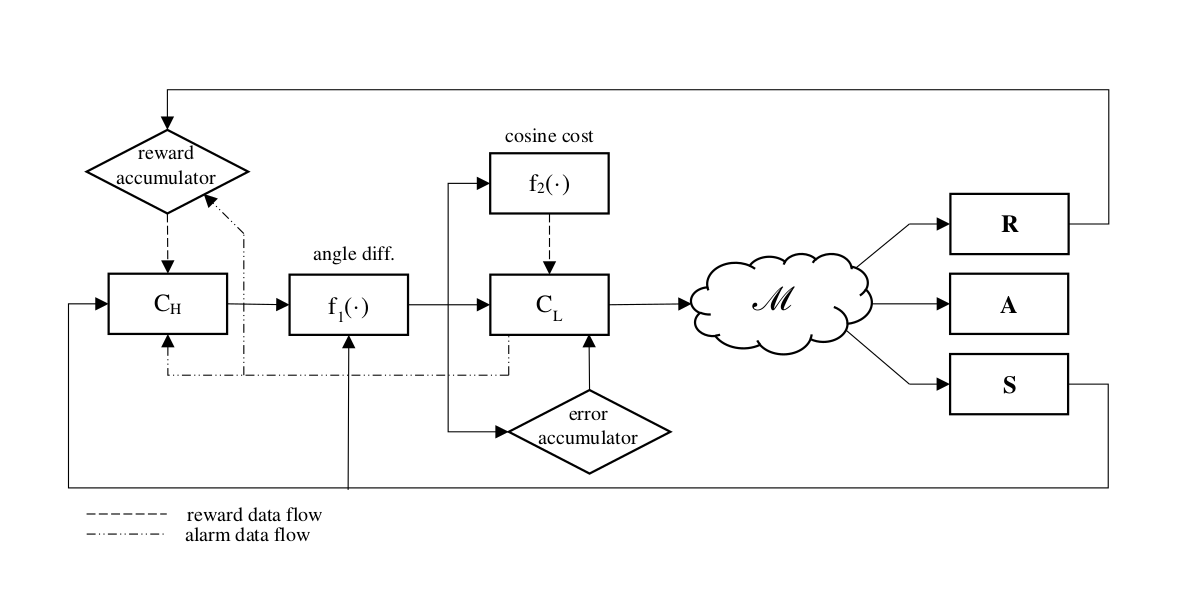
\includegraphics[width = \textwidth]{./pictures/pishipsteering.png}
      \caption{HRL block diagram for ship steering task, PI control action}
      \label{fig:shipsteeringpi}
\end{figure}

 In this case, the state of the low level control is two dimensional. The adopted deterministic policy is $\pi(x) = \left|\boldsymbol{\omega}^T\right|x$. The state vector is $x=\left[\Delta\theta, \int\Delta\theta dt\right]$. The parameter vector is $\boldsymbol{\omega}=\left[K_P, K_I\right]$, where the $K_P$ parameter corresponds to the proportional gain, and the $K_I$ parameter is the integral gain, as they multiply the error and the integral of the error respectively.


\section{Results in Small Domain}

Results of the flat algorithms and of the hierarchical schemes designed with the block diagram approach are compared. 

Figure~\ref{fig:art_J} shows the mean of the objective function for every epoch, averaged for 100 experiments for each algorithm. It shows that flat PG algorithms, i.e., PGPE and GPOMDP, converge much more slowly than the other ones. This is due to the fact that for these algorithms learning rate should be defined. If the learning rate is low, the convergence is slow and if it is too high, learning may be unstable. 

\begin{figure}[t!]
	\centering
    \vspace{-1.0 cm}
    \setlength\figureheight{5.5cm}  
	\setlength\figurewidth{.9\textwidth}
	% This file was created by matplotlib2tikz v0.6.16.
\begin{tikzpicture}

\definecolor{color0}{rgb}{0,0.75,0.75}
\definecolor{color1}{rgb}{0.75,0,0.75}

\begin{axis}[
xlabel={epoch},
ylabel={J},
xmin=-1.25, xmax=26.25,
ymin=-102.045722411051, ymax=-57.2134804981018,
width=\figurewidth,
height=\figureheight,
tick align=outside,
tick pos=left,
x grid style={white!69.01960784313725!black},
y grid style={white!69.01960784313725!black},
legend cell align={left},
legend entries={{H-PGPE},{REPS},{RWR},{PGPE},{GPOMDP}},
legend style={at={(0.97,0.03)}, anchor=south east, draw=white!80.0!black}
]
\addlegendimage{no markers, blue}
\addlegendimage{no markers, red}
\addlegendimage{no markers, green!50.0!black}
\addlegendimage{no markers, color0}
\addlegendimage{no markers, color1}
\path [draw=blue, semithick] (axis cs:0,-100)
--(axis cs:0,-100);

\path [draw=blue, semithick] (axis cs:1,-93.8844031073029)
--(axis cs:1,-95.009392845152);

\path [draw=blue, semithick] (axis cs:2,-92.988679778882)
--(axis cs:2,-94.455724491924);

\path [draw=blue, semithick] (axis cs:3,-89.4770390462373)
--(axis cs:3,-91.5626994845177);

\path [draw=blue, semithick] (axis cs:4,-83.5113933816678)
--(axis cs:4,-86.4362909181087);

\path [draw=blue, semithick] (axis cs:5,-77.4891101370856)
--(axis cs:5,-80.8815692290756);

\path [draw=blue, semithick] (axis cs:6,-71.3979405955427)
--(axis cs:6,-74.5860307612094);

\path [draw=blue, semithick] (axis cs:7,-66.9352745847397)
--(axis cs:7,-70.3229400593475);

\path [draw=blue, semithick] (axis cs:8,-64.5097641964084)
--(axis cs:8,-67.1651054669046);

\path [draw=blue, semithick] (axis cs:9,-62.7616953407986)
--(axis cs:9,-65.3071722033568);

\path [draw=blue, semithick] (axis cs:10,-60.8098074053026)
--(axis cs:10,-62.6421477011409);

\path [draw=blue, semithick] (axis cs:11,-60.9643522984729)
--(axis cs:11,-62.8315185481412);

\path [draw=blue, semithick] (axis cs:12,-60.7362863275358)
--(axis cs:12,-62.430110564971);

\path [draw=blue, semithick] (axis cs:13,-60.3316662413563)
--(axis cs:13,-62.0075482576081);

\path [draw=blue, semithick] (axis cs:14,-59.8101477589761)
--(axis cs:14,-61.2360357577435);

\path [draw=blue, semithick] (axis cs:15,-59.3545994981829)
--(axis cs:15,-60.5245326920989);

\path [draw=blue, semithick] (axis cs:16,-59.9492448417058)
--(axis cs:16,-61.7625818956256);

\path [draw=blue, semithick] (axis cs:17,-59.8445548849395)
--(axis cs:17,-61.1828533442119);

\path [draw=blue, semithick] (axis cs:18,-59.6474778394595)
--(axis cs:18,-61.1941864966046);

\path [draw=blue, semithick] (axis cs:19,-59.6472124838335)
--(axis cs:19,-61.0492925768536);

\path [draw=blue, semithick] (axis cs:20,-59.2523141432313)
--(axis cs:20,-60.1308671855049);

\path [draw=blue, semithick] (axis cs:21,-59.6150564558487)
--(axis cs:21,-60.7430263266553);

\path [draw=blue, semithick] (axis cs:22,-59.479005102806)
--(axis cs:22,-60.8607910312466);

\path [draw=blue, semithick] (axis cs:23,-59.496371057599)
--(axis cs:23,-60.6035422311425);

\path [draw=blue, semithick] (axis cs:24,-59.2513096759631)
--(axis cs:24,-59.8708681188255);

\path [draw=blue, semithick] (axis cs:25,-59.576033041729)
--(axis cs:25,-60.7148514397126);

\path [draw=red, semithick] (axis cs:0,-99.340938091202)
--(axis cs:0,-99.6765177904523);

\path [draw=red, semithick] (axis cs:1,-86.9696915058598)
--(axis cs:1,-91.2842458346257);

\path [draw=red, semithick] (axis cs:2,-70.5203134016048)
--(axis cs:2,-75.3827222086141);

\path [draw=red, semithick] (axis cs:3,-64.609782600434)
--(axis cs:3,-69.0890476554475);

\path [draw=red, semithick] (axis cs:4,-62.7412132718815)
--(axis cs:4,-66.8617231101294);

\path [draw=red, semithick] (axis cs:5,-61.493938772641)
--(axis cs:5,-65.266381187646);

\path [draw=red, semithick] (axis cs:6,-60.9080955761437)
--(axis cs:6,-64.2382385271308);

\path [draw=red, semithick] (axis cs:7,-60.7036473598561)
--(axis cs:7,-63.8902712352318);

\path [draw=red, semithick] (axis cs:8,-60.5440366495401)
--(axis cs:8,-63.7042865629365);

\path [draw=red, semithick] (axis cs:9,-60.5540153114945)
--(axis cs:9,-63.7368389825067);

\path [draw=red, semithick] (axis cs:10,-60.4617134875305)
--(axis cs:10,-63.61971422531);

\path [draw=red, semithick] (axis cs:11,-60.4391637879797)
--(axis cs:11,-63.5985499551863);

\path [draw=red, semithick] (axis cs:12,-60.4784505290768)
--(axis cs:12,-63.638308638653);

\path [draw=red, semithick] (axis cs:13,-60.4382160833601)
--(axis cs:13,-63.597604703527);

\path [draw=red, semithick] (axis cs:14,-60.437790368404)
--(axis cs:14,-63.5972250018576);

\path [draw=red, semithick] (axis cs:15,-60.4381349246686)
--(axis cs:15,-63.5976015659084);

\path [draw=red, semithick] (axis cs:16,-60.437575365644)
--(axis cs:16,-63.5970352726449);

\path [draw=red, semithick] (axis cs:17,-60.4558709663328)
--(axis cs:17,-63.6164633366484);

\path [draw=red, semithick] (axis cs:18,-60.4589820572708)
--(axis cs:18,-63.6168911671207);

\path [draw=red, semithick] (axis cs:19,-60.4381931180551)
--(axis cs:19,-63.597603586875);

\path [draw=red, semithick] (axis cs:20,-60.437575365644)
--(axis cs:20,-63.5970352726449);

\path [draw=red, semithick] (axis cs:21,-60.4585706043821)
--(axis cs:21,-63.6165132311746);

\path [draw=red, semithick] (axis cs:22,-60.437790368404)
--(axis cs:22,-63.5972250018576);

\path [draw=red, semithick] (axis cs:23,-60.45859160974)
--(axis cs:23,-63.6168969577894);

\path [draw=red, semithick] (axis cs:24,-60.4781612401401)
--(axis cs:24,-63.6373798446298);

\path [draw=red, semithick] (axis cs:25,-60.437575365644)
--(axis cs:25,-63.5970352726449);

\path [draw=green!50.0!black, semithick] (axis cs:0,-99.1581387340433)
--(axis cs:0,-99.5481090039911);

\path [draw=green!50.0!black, semithick] (axis cs:1,-80.026635650284)
--(axis cs:1,-85.727121653856);

\path [draw=green!50.0!black, semithick] (axis cs:2,-68.9581863025615)
--(axis cs:2,-73.7213317906966);

\path [draw=green!50.0!black, semithick] (axis cs:3,-65.6956570461768)
--(axis cs:3,-69.9017474993277);

\path [draw=green!50.0!black, semithick] (axis cs:4,-64.1527761758554)
--(axis cs:4,-68.0739174150851);

\path [draw=green!50.0!black, semithick] (axis cs:5,-63.9124984991473)
--(axis cs:5,-67.7846857212685);

\path [draw=green!50.0!black, semithick] (axis cs:6,-63.6743095240205)
--(axis cs:6,-67.5856396425221);

\path [draw=green!50.0!black, semithick] (axis cs:7,-63.2868403376964)
--(axis cs:7,-67.167590915216);

\path [draw=green!50.0!black, semithick] (axis cs:8,-63.3108371629945)
--(axis cs:8,-67.1899199040878);

\path [draw=green!50.0!black, semithick] (axis cs:9,-63.0436749190446)
--(axis cs:9,-66.8795370874546);

\path [draw=green!50.0!black, semithick] (axis cs:10,-62.940045094149)
--(axis cs:10,-66.7690052137587);

\path [draw=green!50.0!black, semithick] (axis cs:11,-62.9508682431492)
--(axis cs:11,-66.7927823215623);

\path [draw=green!50.0!black, semithick] (axis cs:12,-62.9149898808233)
--(axis cs:12,-66.7479361202862);

\path [draw=green!50.0!black, semithick] (axis cs:13,-62.8972913868626)
--(axis cs:13,-66.7356527821435);

\path [draw=green!50.0!black, semithick] (axis cs:14,-62.8596476680646)
--(axis cs:14,-66.7061153537228);

\path [draw=green!50.0!black, semithick] (axis cs:15,-62.8150857558692)
--(axis cs:15,-66.6647303665289);

\path [draw=green!50.0!black, semithick] (axis cs:16,-62.8001270486436)
--(axis cs:16,-66.6445437146755);

\path [draw=green!50.0!black, semithick] (axis cs:17,-62.7960659371176)
--(axis cs:17,-66.6409986224146);

\path [draw=green!50.0!black, semithick] (axis cs:18,-62.7944993351245)
--(axis cs:18,-66.6398571879558);

\path [draw=green!50.0!black, semithick] (axis cs:19,-62.8040224822818)
--(axis cs:19,-66.6541258617261);

\path [draw=green!50.0!black, semithick] (axis cs:20,-62.7917446454782)
--(axis cs:20,-66.6373856247019);

\path [draw=green!50.0!black, semithick] (axis cs:21,-62.7914966359793)
--(axis cs:21,-66.6371982247025);

\path [draw=green!50.0!black, semithick] (axis cs:22,-62.7901516933118)
--(axis cs:22,-66.6357265126988);

\path [draw=green!50.0!black, semithick] (axis cs:23,-62.7901628954246)
--(axis cs:23,-66.6356428053543);

\path [draw=green!50.0!black, semithick] (axis cs:24,-62.7872626927784)
--(axis cs:24,-66.6329665347076);

\path [draw=green!50.0!black, semithick] (axis cs:25,-62.788210241327)
--(axis cs:25,-66.6339829243369);

\path [draw=color0, semithick] (axis cs:0,-99.0619646721375)
--(axis cs:0,-99.4831354500871);

\path [draw=color0, semithick] (axis cs:1,-98.3106370090467)
--(axis cs:1,-98.9810074991301);

\path [draw=color0, semithick] (axis cs:2,-97.3460617668763)
--(axis cs:2,-98.2888480707866);

\path [draw=color0, semithick] (axis cs:3,-97.4688706837659)
--(axis cs:3,-98.3938385676808);

\path [draw=color0, semithick] (axis cs:4,-96.8657939469452)
--(axis cs:4,-97.8956649883799);

\path [draw=color0, semithick] (axis cs:5,-95.8152813951146)
--(axis cs:5,-97.2212870397311);

\path [draw=color0, semithick] (axis cs:6,-93.9069801391457)
--(axis cs:6,-96.2531543992857);

\path [draw=color0, semithick] (axis cs:7,-92.0622529701026)
--(axis cs:7,-94.9835503652816);

\path [draw=color0, semithick] (axis cs:8,-90.2299421160219)
--(axis cs:8,-93.3782156372657);

\path [draw=color0, semithick] (axis cs:9,-87.4518528563457)
--(axis cs:9,-91.439121205612);

\path [draw=color0, semithick] (axis cs:10,-85.5990407286016)
--(axis cs:10,-89.7802831095007);

\path [draw=color0, semithick] (axis cs:11,-82.9871730359104)
--(axis cs:11,-87.3122043760532);

\path [draw=color0, semithick] (axis cs:12,-80.1602801674897)
--(axis cs:12,-85.0907541405663);

\path [draw=color0, semithick] (axis cs:13,-77.6687532958262)
--(axis cs:13,-82.7730378844951);

\path [draw=color0, semithick] (axis cs:14,-77.3360414376375)
--(axis cs:14,-82.374570928434);

\path [draw=color0, semithick] (axis cs:15,-76.1292874116903)
--(axis cs:15,-81.092685861246);

\path [draw=color0, semithick] (axis cs:16,-73.3554848940945)
--(axis cs:16,-78.2353976662902);

\path [draw=color0, semithick] (axis cs:17,-71.6159770142584)
--(axis cs:17,-76.2407043928117);

\path [draw=color0, semithick] (axis cs:18,-70.7060994018115)
--(axis cs:18,-75.1672745242444);

\path [draw=color0, semithick] (axis cs:19,-68.4123756884912)
--(axis cs:19,-72.6687922085187);

\path [draw=color0, semithick] (axis cs:20,-69.0173877575832)
--(axis cs:20,-73.2744772073133);

\path [draw=color0, semithick] (axis cs:21,-67.9647516378067)
--(axis cs:21,-72.0866857228954);

\path [draw=color0, semithick] (axis cs:22,-67.8362160703379)
--(axis cs:22,-71.8738590635436);

\path [draw=color0, semithick] (axis cs:23,-66.8820099408885)
--(axis cs:23,-70.8623854022783);

\path [draw=color0, semithick] (axis cs:24,-66.9736563310659)
--(axis cs:24,-70.947381494199);

\path [draw=color0, semithick] (axis cs:25,-66.0805566543473)
--(axis cs:25,-69.7427805434904);

\path [draw=color1, semithick] (axis cs:0,-100)
--(axis cs:0,-100);

\path [draw=color1, semithick] (axis cs:1,-100)
--(axis cs:1,-100);

\path [draw=color1, semithick] (axis cs:2,-100)
--(axis cs:2,-100);

\path [draw=color1, semithick] (axis cs:3,-99.952238643842)
--(axis cs:3,-100.007893233189);

\path [draw=color1, semithick] (axis cs:4,-99.6687922980591)
--(axis cs:4,-99.8958298484505);

\path [draw=color1, semithick] (axis cs:5,-97.318162989726)
--(axis cs:5,-98.3189864525242);

\path [draw=color1, semithick] (axis cs:6,-88.651116406238)
--(axis cs:6,-90.5252875708918);

\path [draw=color1, semithick] (axis cs:7,-80.1672649149436)
--(axis cs:7,-82.2887325690676);

\path [draw=color1, semithick] (axis cs:8,-75.8331889994754)
--(axis cs:8,-78.1913700213266);

\path [draw=color1, semithick] (axis cs:9,-73.0096915857288)
--(axis cs:9,-75.8144321506643);

\path [draw=color1, semithick] (axis cs:10,-72.2615331925637)
--(axis cs:10,-75.862510531929);

\path [draw=color1, semithick] (axis cs:11,-71.7879776683749)
--(axis cs:11,-76.1357100911378);

\path [draw=color1, semithick] (axis cs:12,-71.6242876833618)
--(axis cs:12,-76.2560728203333);

\path [draw=color1, semithick] (axis cs:13,-71.6977081137204)
--(axis cs:13,-76.6082808676356);

\path [draw=color1, semithick] (axis cs:14,-70.8802098794888)
--(axis cs:14,-76.1488444736344);

\path [draw=color1, semithick] (axis cs:15,-70.6328735103907)
--(axis cs:15,-75.8250122415561);

\path [draw=color1, semithick] (axis cs:16,-69.9444530175129)
--(axis cs:16,-75.2671155368463);

\path [draw=color1, semithick] (axis cs:17,-69.6583132925062)
--(axis cs:17,-75.2366608359157);

\path [draw=color1, semithick] (axis cs:18,-68.7821934875945)
--(axis cs:18,-74.3086194340845);

\path [draw=color1, semithick] (axis cs:19,-69.8921619909389)
--(axis cs:19,-75.6280350506968);

\path [draw=color1, semithick] (axis cs:20,-68.9738249178168)
--(axis cs:20,-74.8222538052091);

\path [draw=color1, semithick] (axis cs:21,-68.8283746083754)
--(axis cs:21,-74.3421208939666);

\path [draw=color1, semithick] (axis cs:22,-68.8095254257202)
--(axis cs:22,-74.5120469067668);

\path [draw=color1, semithick] (axis cs:23,-69.8376351737108)
--(axis cs:23,-75.7269227645284);

\path [draw=color1, semithick] (axis cs:24,-70.7034283224342)
--(axis cs:24,-76.8446793761747);

\path [draw=color1, semithick] (axis cs:25,-70.2978965986904)
--(axis cs:25,-76.4344123547215);

\addplot [semithick, blue, forget plot]
table {%
0 -100
1 -94.4468979762275
2 -93.722202135403
3 -90.5198692653775
4 -84.9738421498883
5 -79.1853396830806
6 -72.9919856783761
7 -68.6291073220436
8 -65.8374348316565
9 -64.0344337720777
10 -61.7259775532218
11 -61.8979354233071
12 -61.5831984462534
13 -61.1696072494822
14 -60.5230917583598
15 -59.9395660951409
16 -60.8559133686657
17 -60.5137041145757
18 -60.420832168032
19 -60.3482525303436
20 -59.6915906643681
21 -60.179041391252
22 -60.1698980670263
23 -60.0499566443707
24 -59.5610888973943
25 -60.1454422407208
};
\addplot [semithick, red, forget plot]
table {%
0 -99.5087279408272
1 -89.1269686702427
2 -72.9515178051095
3 -66.8494151279408
4 -64.8014681910055
5 -63.3801599801435
6 -62.5731670516373
7 -62.296959297544
8 -62.1241616062383
9 -62.1454271470006
10 -62.0407138564202
11 -62.018856871583
12 -62.0583795838649
13 -62.0179103934436
14 -62.0175076851308
15 -62.0178682452885
16 -62.0173053191444
17 -62.0361671514906
18 -62.0379366121957
19 -62.017898352465
20 -62.0173053191444
21 -62.0375419177783
22 -62.0175076851308
23 -62.0377442837647
24 -62.057770542385
25 -62.0173053191444
};
\addplot [semithick, green!50.0!black, forget plot]
table {%
0 -99.3531238690172
1 -82.87687865207
2 -71.339759046629
3 -67.7987022727522
4 -66.1133467954703
5 -65.8485921102079
6 -65.6299745832713
7 -65.2272156264562
8 -65.2503785335412
9 -64.9616060032496
10 -64.8545251539538
11 -64.8718252823557
12 -64.8314630005548
13 -64.816472084503
14 -64.7828815108937
15 -64.739908061199
16 -64.7223353816595
17 -64.7185322797661
18 -64.7171782615401
19 -64.7290741720039
20 -64.7145651350901
21 -64.7143474303409
22 -64.7129391030053
23 -64.7129028503895
24 -64.710114613743
25 -64.7110965828319
};
\addplot [semithick, color0, forget plot]
table {%
0 -99.2725500611123
1 -98.6458222540884
2 -97.8174549188314
3 -97.9313546257234
4 -97.3807294676625
5 -96.5182842174229
6 -95.0800672692157
7 -93.5229016676921
8 -91.8040788766438
9 -89.4454870309788
10 -87.6896619190511
11 -85.1496887059818
12 -82.625517154028
13 -80.2208955901606
14 -79.8553061830358
15 -78.6109866364681
16 -75.7954412801923
17 -73.9283407035351
18 -72.9366869630279
19 -70.5405839485049
20 -71.1459324824483
21 -70.0257186803511
22 -69.8550375669408
23 -68.8721976715834
24 -68.9605189126324
25 -67.9116685989188
};
\addplot [semithick, color1, forget plot]
table {%
0 -100
1 -100
2 -100
3 -99.9800659385157
4 -99.7823110732548
5 -97.8185747211251
6 -89.5882019885649
7 -81.2279987420056
8 -77.012279510401
9 -74.4120618681966
10 -74.0620218622463
11 -73.9618438797563
12 -73.9401802518475
13 -74.152994490678
14 -73.5145271765616
15 -73.2289428759734
16 -72.6057842771796
17 -72.4474870642109
18 -71.5454064608395
19 -72.7600985208178
20 -71.8980393615129
21 -71.585247751171
22 -71.6607861662435
23 -72.7822789691196
24 -73.7740538493045
25 -73.3661544767059
};
\end{axis}

\end{tikzpicture}
    \caption[J comparison, hierarchical vs. flat, small environment]{Comparison of the hierarchical structure w.r.t. flat policy search for small environment. Mean values of objective functions with 95\% confidence intervals are shown}
    \label{fig:art_J}
\end{figure} 

\begin{figure}[t!]
	\centering
	\setlength\figureheight{5.5cm}  
	\setlength\figurewidth{.9\textwidth}
	% This file was created by matplotlib2tikz v0.6.16.
\begin{tikzpicture}

\definecolor{color0}{rgb}{0,0.75,0.75}
\definecolor{color1}{rgb}{0.75,0,0.75}

\begin{axis}[
xlabel={epoch},
ylabel={episode length},
xmin=-1.25, xmax=26.25,
ymin=10.7311004140636, ymax=222.739277592819,
width=\figurewidth,
height=\figureheight,
tick align=outside,
tick pos=left,
x grid style={white!69.01960784313725!black},
y grid style={white!69.01960784313725!black}
]
\path [draw=red, semithick] (axis cs:0,77.6465189830409)
--(axis cs:0,51.6534810169591);

\path [draw=red, semithick] (axis cs:1,132.95882663092)
--(axis cs:1,99.2901733690802);

\path [draw=red, semithick] (axis cs:2,120.533846588516)
--(axis cs:2,95.0331534114837);

\path [draw=red, semithick] (axis cs:3,112.867854818109)
--(axis cs:3,91.2051451818911);

\path [draw=red, semithick] (axis cs:4,94.9615444848637)
--(axis cs:4,86.7604555151364);

\path [draw=red, semithick] (axis cs:5,93.0931087223105)
--(axis cs:5,85.5778912776895);

\path [draw=red, semithick] (axis cs:6,93.0077444511953)
--(axis cs:6,85.3612555488048);

\path [draw=red, semithick] (axis cs:7,92.9470953640859)
--(axis cs:7,85.3619046359141);

\path [draw=red, semithick] (axis cs:8,92.5339966898285)
--(axis cs:8,85.0670033101715);

\path [draw=red, semithick] (axis cs:9,92.4850876831196)
--(axis cs:9,85.0389123168804);

\path [draw=red, semithick] (axis cs:10,92.416308064436)
--(axis cs:10,84.982691935564);

\path [draw=red, semithick] (axis cs:11,92.3791790969445)
--(axis cs:11,84.9488209030555);

\path [draw=red, semithick] (axis cs:12,92.3994425049658)
--(axis cs:12,84.9675574950343);

\path [draw=red, semithick] (axis cs:13,92.3764654773029)
--(axis cs:13,84.9465345226971);

\path [draw=red, semithick] (axis cs:14,92.3754452554255)
--(axis cs:14,84.9455547445745);

\path [draw=red, semithick] (axis cs:15,92.3765778785328)
--(axis cs:15,84.9464221214672);

\path [draw=red, semithick] (axis cs:16,92.3749379505262)
--(axis cs:16,84.9450620494738);

\path [draw=red, semithick] (axis cs:17,92.3842350365168)
--(axis cs:17,84.9527649634832);

\path [draw=red, semithick] (axis cs:18,92.3861705601554)
--(axis cs:18,84.9558294398446);

\path [draw=red, semithick] (axis cs:19,92.3764927750571)
--(axis cs:19,84.9465072249429);

\path [draw=red, semithick] (axis cs:20,92.3749379505262)
--(axis cs:20,84.9450620494738);

\path [draw=red, semithick] (axis cs:21,92.3851343842904)
--(axis cs:21,84.9548656157096);

\path [draw=red, semithick] (axis cs:22,92.3754452554255)
--(axis cs:22,84.9455547445745);

\path [draw=red, semithick] (axis cs:23,92.3930101954929)
--(axis cs:23,84.9619898045071);

\path [draw=red, semithick] (axis cs:24,92.4087882564084)
--(axis cs:24,84.9762117435916);

\path [draw=red, semithick] (axis cs:25,92.3749379505262)
--(axis cs:25,84.9450620494738);

\path [draw=green!50.0!black, semithick] (axis cs:0,60.8651875108613)
--(axis cs:0,42.0718124891387);

\path [draw=green!50.0!black, semithick] (axis cs:1,182.25297394911)
--(axis cs:1,100.48702605089);

\path [draw=green!50.0!black, semithick] (axis cs:2,118.641823995237)
--(axis cs:2,95.4721760047635);

\path [draw=green!50.0!black, semithick] (axis cs:3,108.545900866808)
--(axis cs:3,93.3440991331921);

\path [draw=green!50.0!black, semithick] (axis cs:4,102.437951277028)
--(axis cs:4,92.369048722972);

\path [draw=green!50.0!black, semithick] (axis cs:5,100.556307093505)
--(axis cs:5,91.3986929064948);

\path [draw=green!50.0!black, semithick] (axis cs:6,100.619416881768)
--(axis cs:6,90.9005831182324);

\path [draw=green!50.0!black, semithick] (axis cs:7,99.3799686252515)
--(axis cs:7,90.0980313747486);

\path [draw=green!50.0!black, semithick] (axis cs:8,98.7866759307523)
--(axis cs:8,89.7463240692476);

\path [draw=green!50.0!black, semithick] (axis cs:9,98.2677759815255)
--(axis cs:9,89.4232240184745);

\path [draw=green!50.0!black, semithick] (axis cs:10,98.1118224535946)
--(axis cs:10,89.2841775464054);

\path [draw=green!50.0!black, semithick] (axis cs:11,98.0939489496351)
--(axis cs:11,89.272051050365);

\path [draw=green!50.0!black, semithick] (axis cs:12,98.0872091542537)
--(axis cs:12,89.3527908457464);

\path [draw=green!50.0!black, semithick] (axis cs:13,97.9930602107108)
--(axis cs:13,89.1929397892893);

\path [draw=green!50.0!black, semithick] (axis cs:14,98.1080772499006)
--(axis cs:14,89.3669227500994);

\path [draw=green!50.0!black, semithick] (axis cs:15,98.0821621066667)
--(axis cs:15,89.2898378933333);

\path [draw=green!50.0!black, semithick] (axis cs:16,98.0746563063124)
--(axis cs:16,89.3993436936876);

\path [draw=green!50.0!black, semithick] (axis cs:17,97.9062121188145)
--(axis cs:17,89.1697878811855);

\path [draw=green!50.0!black, semithick] (axis cs:18,97.9784148007049)
--(axis cs:18,89.2725851992951);

\path [draw=green!50.0!black, semithick] (axis cs:19,97.8488204176464)
--(axis cs:19,89.0641795823536);

\path [draw=green!50.0!black, semithick] (axis cs:20,97.8602608705338)
--(axis cs:20,89.0607391294662);

\path [draw=green!50.0!black, semithick] (axis cs:21,97.8667198130308)
--(axis cs:21,89.0802801869692);

\path [draw=green!50.0!black, semithick] (axis cs:22,97.8606359486784)
--(axis cs:22,89.0723640513217);

\path [draw=green!50.0!black, semithick] (axis cs:23,97.862808040035)
--(axis cs:23,89.079191959965);

\path [draw=green!50.0!black, semithick] (axis cs:24,97.8491595344612)
--(axis cs:24,89.0548404655388);

\path [draw=green!50.0!black, semithick] (axis cs:25,97.8525532777812)
--(axis cs:25,89.0564467222188);

\path [draw=color0, semithick] (axis cs:0,58.6739676813791)
--(axis cs:0,40.981032318621);

\path [draw=color0, semithick] (axis cs:1,98.5531830010912)
--(axis cs:1,69.4728169989089);

\path [draw=color0, semithick] (axis cs:2,117.34547410334)
--(axis cs:2,88.5695258966596);

\path [draw=color0, semithick] (axis cs:3,125.08083419636)
--(axis cs:3,86.8891658036401);

\path [draw=color0, semithick] (axis cs:4,137.021548491112)
--(axis cs:4,93.460451508888);

\path [draw=color0, semithick] (axis cs:5,136.163290174894)
--(axis cs:5,98.9697098251064);

\path [draw=color0, semithick] (axis cs:6,146.838746390793)
--(axis cs:6,106.331253609207);

\path [draw=color0, semithick] (axis cs:7,213.102542266512)
--(axis cs:7,147.139457733488);

\path [draw=color0, semithick] (axis cs:8,188.204052029609)
--(axis cs:8,127.532947970391);

\path [draw=color0, semithick] (axis cs:9,181.306832053566)
--(axis cs:9,126.647167946434);

\path [draw=color0, semithick] (axis cs:10,179.112766892413)
--(axis cs:10,130.204233107587);

\path [draw=color0, semithick] (axis cs:11,139.883755119949)
--(axis cs:11,108.553244880051);

\path [draw=color0, semithick] (axis cs:12,162.765558617036)
--(axis cs:12,117.172441382964);

\path [draw=color0, semithick] (axis cs:13,142.985640891854)
--(axis cs:13,101.623359108146);

\path [draw=color0, semithick] (axis cs:14,163.520860279532)
--(axis cs:14,118.675139720468);

\path [draw=color0, semithick] (axis cs:15,140.421634383614)
--(axis cs:15,106.712365616387);

\path [draw=color0, semithick] (axis cs:16,129.13858499695)
--(axis cs:16,102.47641500305);

\path [draw=color0, semithick] (axis cs:17,155.358365559882)
--(axis cs:17,113.864634440118);

\path [draw=color0, semithick] (axis cs:18,132.303074186424)
--(axis cs:18,101.799925813576);

\path [draw=color0, semithick] (axis cs:19,137.810430711711)
--(axis cs:19,107.758569288289);

\path [draw=color0, semithick] (axis cs:20,112.884480976539)
--(axis cs:20,96.177519023461);

\path [draw=color0, semithick] (axis cs:21,117.614642761054)
--(axis cs:21,97.2443572389459);

\path [draw=color0, semithick] (axis cs:22,123.869795814105)
--(axis cs:22,98.4102041858948);

\path [draw=color0, semithick] (axis cs:23,126.584772340975)
--(axis cs:23,100.519227659025);

\path [draw=color0, semithick] (axis cs:24,130.813842725717)
--(axis cs:24,95.3691572742829);

\path [draw=color0, semithick] (axis cs:25,116.662834362606)
--(axis cs:25,95.7971656373938);

\path [draw=color1, semithick] (axis cs:0,22.3296642596294)
--(axis cs:0,20.3678357403706);

\path [draw=color1, semithick] (axis cs:1,47.2991810560451)
--(axis cs:1,44.7553189439549);

\path [draw=color1, semithick] (axis cs:2,65.0480631989726)
--(axis cs:2,61.7659368010274);

\path [draw=color1, semithick] (axis cs:3,78.3805289775063)
--(axis cs:3,75.4649710224937);

\path [draw=color1, semithick] (axis cs:4,90.4072150385205)
--(axis cs:4,87.3827849614795);

\path [draw=color1, semithick] (axis cs:5,101.831597232978)
--(axis cs:5,99.2744027670222);

\path [draw=color1, semithick] (axis cs:6,106.298238261914)
--(axis cs:6,103.195761738086);

\path [draw=color1, semithick] (axis cs:7,104.765819147167)
--(axis cs:7,102.392680852833);

\path [draw=color1, semithick] (axis cs:8,102.596389814168)
--(axis cs:8,100.086610185832);

\path [draw=color1, semithick] (axis cs:9,102.036169565835)
--(axis cs:9,99.5243304341652);

\path [draw=color1, semithick] (axis cs:10,102.449630761042)
--(axis cs:10,99.275369238958);

\path [draw=color1, semithick] (axis cs:11,103.316265490052)
--(axis cs:11,99.6602345099477);

\path [draw=color1, semithick] (axis cs:12,103.962190828174)
--(axis cs:12,100.151309171826);

\path [draw=color1, semithick] (axis cs:13,104.592408749368)
--(axis cs:13,100.588091250632);

\path [draw=color1, semithick] (axis cs:14,103.716922666702)
--(axis cs:14,99.3410773332981);

\path [draw=color1, semithick] (axis cs:15,103.984594461716)
--(axis cs:15,99.6704055382841);

\path [draw=color1, semithick] (axis cs:16,103.578054509815)
--(axis cs:16,99.146945490185);

\path [draw=color1, semithick] (axis cs:17,103.740613770618)
--(axis cs:17,99.1148862293819);

\path [draw=color1, semithick] (axis cs:18,102.989272313465)
--(axis cs:18,98.3557276865355);

\path [draw=color1, semithick] (axis cs:19,104.196937010045)
--(axis cs:19,99.4385629899553);

\path [draw=color1, semithick] (axis cs:20,103.907739869036)
--(axis cs:20,99.0057601309638);

\path [draw=color1, semithick] (axis cs:21,103.363348470393)
--(axis cs:21,98.7891515296074);

\path [draw=color1, semithick] (axis cs:22,103.786621635631)
--(axis cs:22,98.9673783643689);

\path [draw=color1, semithick] (axis cs:23,104.549489501946)
--(axis cs:23,99.5845104980539);

\path [draw=color1, semithick] (axis cs:24,105.511104762414)
--(axis cs:24,100.378895237586);

\path [draw=color1, semithick] (axis cs:25,105.397228599543)
--(axis cs:25,100.336771400458);

\addplot [semithick, red, forget plot]
table {%
0 64.65
1 116.1245
2 107.7835
3 102.0365
4 90.861
5 89.3355
6 89.1845
7 89.1545
8 88.8005
9 88.762
10 88.6995
11 88.664
12 88.6835
13 88.6615
14 88.6605
15 88.6615
16 88.66
17 88.6685
18 88.671
19 88.6615
20 88.66
21 88.67
22 88.6605
23 88.6775
24 88.6925
25 88.66
};
\addplot [semithick, green!50.0!black, forget plot]
table {%
0 51.4685
1 141.37
2 107.057
3 100.945
4 97.4035
5 95.9775
6 95.76
7 94.739
8 94.2665
9 93.8455
10 93.698
11 93.683
12 93.72
13 93.593
14 93.7375
15 93.686
16 93.737
17 93.538
18 93.6255
19 93.4565
20 93.4605
21 93.4735
22 93.4665
23 93.471
24 93.452
25 93.4545
};
\addplot [semithick, color0, forget plot]
table {%
0 49.8275
1 84.013
2 102.9575
3 105.985
4 115.241
5 117.5665
6 126.585
7 180.121
8 157.8685
9 153.977
10 154.6585
11 124.2185
12 139.969
13 122.3045
14 141.098
15 123.567
16 115.8075
17 134.6115
18 117.0515
19 122.7845
20 104.531
21 107.4295
22 111.14
23 113.552
24 113.0915
25 106.23
};
\addplot [semithick, color1, forget plot]
table {%
0 21.34875
1 46.02725
2 63.407
3 76.92275
4 88.895
5 100.553
6 104.747
7 103.57925
8 101.3415
9 100.78025
10 100.8625
11 101.48825
12 102.05675
13 102.59025
14 101.529
15 101.8275
16 101.3625
17 101.42775
18 100.6725
19 101.81775
20 101.45675
21 101.07625
22 101.377
23 102.067
24 102.945
25 102.867
};
\end{axis}

\end{tikzpicture}
    \caption[Epiosde length comparison, flat algorithms, small environment]{Comparison between flat policy search algorithms for small environment. Mean values of episode lengths with 95\% confidence intervals are shown}
    	\label{fig:art_j}
\end{figure}
\begin{figure}[t!]
	\centering
    \setlength\figureheight{5.5cm}  
	\setlength\figurewidth{.9\textwidth}
	% This file was created by matplotlib2tikz v0.6.16.
\begin{tikzpicture}

\begin{axis}[
xlabel={epoch},
ylabel={episode length},
xmin=-1.25, xmax=26.25,
ymin=-0.176985705582929, ymax=1140.09328219034,
width=\figurewidth,
height=\figureheight,
tick align=outside,
tick pos=left,
x grid style={white!69.01960784313725!black},
y grid style={white!69.01960784313725!black}
]
\path [draw=blue, semithick] (axis cs:0,81.0911760668363)
--(axis cs:0,79.7708239331638);

\path [draw=blue, semithick] (axis cs:1,489.404089545043)
--(axis cs:1,426.197910454957);

\path [draw=blue, semithick] (axis cs:2,1088.2628154678)
--(axis cs:2,883.186184532202);

\path [draw=blue, semithick] (axis cs:3,902.729243554014)
--(axis cs:3,668.031756445986);

\path [draw=blue, semithick] (axis cs:4,538.649445355297)
--(axis cs:4,388.479554644704);

\path [draw=blue, semithick] (axis cs:5,360.585648488226)
--(axis cs:5,256.607351511774);

\path [draw=blue, semithick] (axis cs:6,206.965204754822)
--(axis cs:6,168.017795245178);

\path [draw=blue, semithick] (axis cs:7,169.231441872846)
--(axis cs:7,133.929558127155);

\path [draw=blue, semithick] (axis cs:8,133.475028224666)
--(axis cs:8,114.202971775334);

\path [draw=blue, semithick] (axis cs:9,120.197500073287)
--(axis cs:9,102.460499926713);

\path [draw=blue, semithick] (axis cs:10,104.727491148319)
--(axis cs:10,94.9935088516812);

\path [draw=blue, semithick] (axis cs:11,108.924620800781)
--(axis cs:11,95.2993791992188);

\path [draw=blue, semithick] (axis cs:12,104.255991538558)
--(axis cs:12,93.2330084614424);

\path [draw=blue, semithick] (axis cs:13,98.0292641895068)
--(axis cs:13,92.0547358104933);

\path [draw=blue, semithick] (axis cs:14,98.8711748590563)
--(axis cs:14,90.1158251409437);

\path [draw=blue, semithick] (axis cs:15,93.3654467977495)
--(axis cs:15,89.5665532022504);

\path [draw=blue, semithick] (axis cs:16,97.5575558096076)
--(axis cs:16,90.2624441903923);

\path [draw=blue, semithick] (axis cs:17,97.9323236248251)
--(axis cs:17,91.0486763751749);

\path [draw=blue, semithick] (axis cs:18,95.5247837818183)
--(axis cs:18,90.2502162181817);

\path [draw=blue, semithick] (axis cs:19,94.023289405138)
--(axis cs:19,89.856710594862);

\path [draw=blue, semithick] (axis cs:20,92.2067689802821)
--(axis cs:20,89.3982310197179);

\path [draw=blue, semithick] (axis cs:21,93.391101891151)
--(axis cs:21,89.895898108849);

\path [draw=blue, semithick] (axis cs:22,93.3524553428036)
--(axis cs:22,90.0975446571963);

\path [draw=blue, semithick] (axis cs:23,97.7341276584202)
--(axis cs:23,88.6568723415798);

\path [draw=blue, semithick] (axis cs:24,90.3209027734668)
--(axis cs:24,88.8900972265332);

\path [draw=blue, semithick] (axis cs:25,92.5221037823311)
--(axis cs:25,89.4808962176688);

\path [draw=red, semithick] (axis cs:0,77.6465189830409)
--(axis cs:0,51.6534810169591);

\path [draw=red, semithick] (axis cs:1,132.95882663092)
--(axis cs:1,99.2901733690802);

\path [draw=red, semithick] (axis cs:2,120.533846588516)
--(axis cs:2,95.0331534114837);

\path [draw=red, semithick] (axis cs:3,112.867854818109)
--(axis cs:3,91.2051451818911);

\path [draw=red, semithick] (axis cs:4,94.9615444848637)
--(axis cs:4,86.7604555151364);

\path [draw=red, semithick] (axis cs:5,93.0931087223105)
--(axis cs:5,85.5778912776895);

\path [draw=red, semithick] (axis cs:6,93.0077444511953)
--(axis cs:6,85.3612555488048);

\path [draw=red, semithick] (axis cs:7,92.9470953640859)
--(axis cs:7,85.3619046359141);

\path [draw=red, semithick] (axis cs:8,92.5339966898285)
--(axis cs:8,85.0670033101715);

\path [draw=red, semithick] (axis cs:9,92.4850876831196)
--(axis cs:9,85.0389123168804);

\path [draw=red, semithick] (axis cs:10,92.416308064436)
--(axis cs:10,84.982691935564);

\path [draw=red, semithick] (axis cs:11,92.3791790969445)
--(axis cs:11,84.9488209030555);

\path [draw=red, semithick] (axis cs:12,92.3994425049658)
--(axis cs:12,84.9675574950343);

\path [draw=red, semithick] (axis cs:13,92.3764654773029)
--(axis cs:13,84.9465345226971);

\path [draw=red, semithick] (axis cs:14,92.3754452554255)
--(axis cs:14,84.9455547445745);

\path [draw=red, semithick] (axis cs:15,92.3765778785328)
--(axis cs:15,84.9464221214672);

\path [draw=red, semithick] (axis cs:16,92.3749379505262)
--(axis cs:16,84.9450620494738);

\path [draw=red, semithick] (axis cs:17,92.3842350365168)
--(axis cs:17,84.9527649634832);

\path [draw=red, semithick] (axis cs:18,92.3861705601554)
--(axis cs:18,84.9558294398446);

\path [draw=red, semithick] (axis cs:19,92.3764927750571)
--(axis cs:19,84.9465072249429);

\path [draw=red, semithick] (axis cs:20,92.3749379505262)
--(axis cs:20,84.9450620494738);

\path [draw=red, semithick] (axis cs:21,92.3851343842904)
--(axis cs:21,84.9548656157096);

\path [draw=red, semithick] (axis cs:22,92.3754452554255)
--(axis cs:22,84.9455547445745);

\path [draw=red, semithick] (axis cs:23,92.3930101954929)
--(axis cs:23,84.9619898045071);

\path [draw=red, semithick] (axis cs:24,92.4087882564084)
--(axis cs:24,84.9762117435916);

\path [draw=red, semithick] (axis cs:25,92.3749379505262)
--(axis cs:25,84.9450620494738);

\addplot [semithick, blue, forget plot]
table {%
0 80.4310000000001
1 457.801
2 985.7245
3 785.3805
4 463.5645
5 308.5965
6 187.4915
7 151.5805
8 123.839
9 111.329
10 99.8605
11 102.112
12 98.7445
13 95.042
14 94.4935
15 91.466
16 93.91
17 94.4905
18 92.8875
19 91.94
20 90.8025
21 91.6435
22 91.725
23 93.1955
24 89.6055
25 91.0015
};
\addplot [semithick, red, forget plot]
table {%
0 64.65
1 116.1245
2 107.7835
3 102.0365
4 90.861
5 89.3355
6 89.1845
7 89.1545
8 88.8005
9 88.762
10 88.6995
11 88.664
12 88.6835
13 88.6615
14 88.6605
15 88.6615
16 88.66
17 88.6685
18 88.671
19 88.6615
20 88.66
21 88.67
22 88.6605
23 88.6775
24 88.6925
25 88.66
};
\end{axis}

\end{tikzpicture}
    \caption[J comparison, flat vs. hierarchical, small environment]{Comparison of the hierarchical structure w.r.t. flat policy search for small environment. Mean values of episode lengths with 95\% confidence intervals are shown}
    	\label{fig:comp_art_l}
\end{figure}

Figure~\ref{fig:art_j} and Figure~\ref{fig:comp_art_l} show the mean length of the episodes for each epoch, averaged for 100 experiments for different algorithms. Hierarchical algorithm has a large episode length for the first runs. Since the controller is stable, it learns first to avoid to get out of the boundaries, which causes the long episodes exploring the middle of the map. Once the gate is identified well, the shortest path is approximated, which results in gradually lowered episode lengths. 

\begin{figure}[t!]
	\centering
    \setlength\figureheight{6cm}  
	\setlength\figurewidth{\textwidth}
	% This file was created by matplotlib2tikz v0.6.16.
\begin{tikzpicture}

\definecolor{color0}{rgb}{1,0.498039215686275,0.0549019607843137}

\begin{axis}[
xlabel={epoch},
ylabel={J},
xmin=-1.25, xmax=26.25,
ymin=-99.6868135838367, ymax=-86.1646488743638,
width=\figurewidth,
height=\figureheight,
tick align=outside,
tick pos=left,
ytick distance=2,
x grid style={white!69.01960784313725!black},
y grid style={white!69.01960784313725!black},
legend style={at={(0.03,0.97)}, anchor=north west, draw=white!80.0!black, font=\footnotesize},
legend cell align={left},
legend entries={{H-PGPE},{H-PI}}
]
\addlegendimage{no markers, blue}
\addlegendimage{no markers, color0}
\path [draw=blue, semithick] (axis cs:0,-98.6186432917592)
--(axis cs:0,-99.0721697334062);

\path [draw=blue, semithick] (axis cs:1,-97.3191400856202)
--(axis cs:1,-97.8178021915616);

\path [draw=blue, semithick] (axis cs:2,-97.3278734543125)
--(axis cs:2,-97.8491522869482);

\path [draw=blue, semithick] (axis cs:3,-96.4883726412631)
--(axis cs:3,-97.0522423665752);

\path [draw=blue, semithick] (axis cs:4,-95.3321362008732)
--(axis cs:4,-95.9618640658969);

\path [draw=blue, semithick] (axis cs:5,-93.2854433247004)
--(axis cs:5,-94.043623644619);

\path [draw=blue, semithick] (axis cs:6,-92.0833272273029)
--(axis cs:6,-93.0380850103506);

\path [draw=blue, semithick] (axis cs:7,-91.7688697330869)
--(axis cs:7,-92.640125764855);

\path [draw=blue, semithick] (axis cs:8,-91.4295546914821)
--(axis cs:8,-92.3550538777955);

\path [draw=blue, semithick] (axis cs:9,-90.1366372529003)
--(axis cs:9,-91.1408314789972);

\path [draw=blue, semithick] (axis cs:10,-89.3819097193017)
--(axis cs:10,-90.4569828250573);

\path [draw=blue, semithick] (axis cs:11,-88.6623202015229)
--(axis cs:11,-89.7871428591142);

\path [draw=blue, semithick] (axis cs:12,-88.2028771930043)
--(axis cs:12,-89.2885220246916);

\path [draw=blue, semithick] (axis cs:13,-88.0382573414197)
--(axis cs:13,-88.958562559077);

\path [draw=blue, semithick] (axis cs:14,-87.8354842344783)
--(axis cs:14,-88.7056492880469);

\path [draw=blue, semithick] (axis cs:15,-87.6855425682927)
--(axis cs:15,-88.5232913132147);

\path [draw=blue, semithick] (axis cs:16,-87.4473870237435)
--(axis cs:16,-88.2740763683597);

\path [draw=blue, semithick] (axis cs:17,-87.2568090777906)
--(axis cs:17,-88.0484866995881);

\path [draw=blue, semithick] (axis cs:18,-86.7792927247944)
--(axis cs:18,-87.7952475818047);

\path [draw=blue, semithick] (axis cs:19,-87.5104602783067)
--(axis cs:19,-88.288098992873);

\path [draw=blue, semithick] (axis cs:20,-87.1507000685934)
--(axis cs:20,-87.8272381042379);

\path [draw=blue, semithick] (axis cs:21,-86.8388083556658)
--(axis cs:21,-87.6314974459656);

\path [draw=blue, semithick] (axis cs:22,-87.0965359404103)
--(axis cs:22,-87.9233301161857);

\path [draw=blue, semithick] (axis cs:23,-87.0477044536614)
--(axis cs:23,-87.97837387626);

\path [draw=blue, semithick] (axis cs:24,-87.194786281133)
--(axis cs:24,-87.9462999653316);

\path [draw=blue, semithick] (axis cs:25,-87.2897392480625)
--(axis cs:25,-88.1143129161197);

\path [draw=color0, semithick] (axis cs:0,-98.5796385537277)
--(axis cs:0,-99.0309306475881);

\path [draw=color0, semithick] (axis cs:1,-97.5716316566127)
--(axis cs:1,-97.9918288268185);

\path [draw=color0, semithick] (axis cs:2,-97.0669784243078)
--(axis cs:2,-97.501113678087);

\path [draw=color0, semithick] (axis cs:3,-96.2342627825226)
--(axis cs:3,-96.7869267961619);

\path [draw=color0, semithick] (axis cs:4,-95.0329235446257)
--(axis cs:4,-95.7222100807895);

\path [draw=color0, semithick] (axis cs:5,-93.0937192877062)
--(axis cs:5,-93.8776043635349);

\path [draw=color0, semithick] (axis cs:6,-92.3350837476444)
--(axis cs:6,-93.0417769459607);

\path [draw=color0, semithick] (axis cs:7,-91.4788770484909)
--(axis cs:7,-92.3417237709249);

\path [draw=color0, semithick] (axis cs:8,-91.1310097701006)
--(axis cs:8,-92.047568338441);

\path [draw=color0, semithick] (axis cs:9,-90.4633856769803)
--(axis cs:9,-91.4919649627105);

\path [draw=color0, semithick] (axis cs:10,-89.4641388867949)
--(axis cs:10,-90.4410040316289);

\path [draw=color0, semithick] (axis cs:11,-88.7338270291225)
--(axis cs:11,-89.8049259445917);

\path [draw=color0, semithick] (axis cs:12,-88.072036361087)
--(axis cs:12,-89.075977943898);

\path [draw=color0, semithick] (axis cs:13,-88.0334231036403)
--(axis cs:13,-88.9630553438613);

\path [draw=color0, semithick] (axis cs:14,-87.5037462720889)
--(axis cs:14,-88.4244122807454);

\path [draw=color0, semithick] (axis cs:15,-87.6603391279723)
--(axis cs:15,-88.4998572973396);

\path [draw=color0, semithick] (axis cs:16,-87.3362260245575)
--(axis cs:16,-88.0921312903672);

\path [draw=color0, semithick] (axis cs:17,-87.2567126703445)
--(axis cs:17,-88.0716591757684);

\path [draw=color0, semithick] (axis cs:18,-87.1310731076264)
--(axis cs:18,-88.0129853278574);

\path [draw=color0, semithick] (axis cs:19,-86.960662621279)
--(axis cs:19,-87.7342131976424);

\path [draw=color0, semithick] (axis cs:20,-87.4994605608238)
--(axis cs:20,-88.2187986048138);

\path [draw=color0, semithick] (axis cs:21,-86.9885281246732)
--(axis cs:21,-87.8190471228839);

\path [draw=color0, semithick] (axis cs:22,-87.1373384630533)
--(axis cs:22,-87.8540316644523);

\path [draw=color0, semithick] (axis cs:23,-87.320752285901)
--(axis cs:23,-88.0645632405074);

\path [draw=color0, semithick] (axis cs:24,-86.9449738682615)
--(axis cs:24,-87.8696912413971);

\path [draw=color0, semithick] (axis cs:25,-87.3435372012375)
--(axis cs:25,-88.1321930489828);

\addplot [semithick, blue, forget plot]
table {%
0 -98.8454065125827
1 -97.5684711385909
2 -97.5885128706303
3 -96.7703075039191
4 -95.6470001333851
5 -93.6645334846597
6 -92.5607061188267
7 -92.2044977489709
8 -91.8923042846388
9 -90.6387343659487
10 -89.9194462721795
11 -89.2247315303186
12 -88.745699608848
13 -88.4984099502484
14 -88.2705667612626
15 -88.1044169407537
16 -87.8607316960516
17 -87.6526478886894
18 -87.2872701532995
19 -87.8992796355898
20 -87.4889690864157
21 -87.2351529008157
22 -87.509933028298
23 -87.5130391649607
24 -87.5705431232323
25 -87.7020260820911
};
\addplot [semithick, color0, forget plot]
table {%
0 -98.8052846006579
1 -97.7817302417156
2 -97.2840460511974
3 -96.5105947893422
4 -95.3775668127076
5 -93.4856618256205
6 -92.6884303468026
7 -91.9103004097079
8 -91.5892890542708
9 -90.9776753198454
10 -89.9525714592119
11 -89.2693764868571
12 -88.5740071524925
13 -88.4982392237508
14 -87.9640792764171
15 -88.0800982126559
16 -87.7141786574624
17 -87.6641859230565
18 -87.5720292177419
19 -87.3474379094607
20 -87.8591295828188
21 -87.4037876237786
22 -87.4956850637528
23 -87.6926577632042
24 -87.4073325548293
25 -87.7378651251101
};
\end{axis}

\end{tikzpicture}
    \caption[J comparison, hierarchical algorithms, small environment]{Comparison between the hierarchical structures search for small environment. Mean values of objective functions with 95\% confidence intervals are shown}
    \label{fig:hier_J}
\end{figure}
\begin{figure}[t!]
	\centering
    \setlength\figureheight{6cm}  
	\setlength\figurewidth{\textwidth}
	% This file was created by matplotlib2tikz v0.6.16.
\begin{tikzpicture}

\definecolor{color0}{rgb}{1,0.498039215686275,0.0549019607843137}
\definecolor{color1}{rgb}{0.580392156862745,0.403921568627451,0.741176470588235}

\begin{axis}[
xlabel={epoch},
ylabel={episode length},
xmin=-1.25, xmax=26.25,
ymin=-34.915452394257, ymax=1141.7474948898,
width=\figurewidth,
height=\figureheight,
tick align=outside,
tick pos=left,
x grid style={white!69.01960784313725!black},
y grid style={white!69.01960784313725!black}
]
\path [draw=blue, semithick] (axis cs:0,81.0911760668363)
--(axis cs:0,79.7708239331638);

\path [draw=blue, semithick] (axis cs:1,489.404089545043)
--(axis cs:1,426.197910454957);

\path [draw=blue, semithick] (axis cs:2,1088.2628154678)
--(axis cs:2,883.186184532202);

\path [draw=blue, semithick] (axis cs:3,902.729243554014)
--(axis cs:3,668.031756445986);

\path [draw=blue, semithick] (axis cs:4,538.649445355297)
--(axis cs:4,388.479554644704);

\path [draw=blue, semithick] (axis cs:5,360.585648488226)
--(axis cs:5,256.607351511774);

\path [draw=blue, semithick] (axis cs:6,206.965204754822)
--(axis cs:6,168.017795245178);

\path [draw=blue, semithick] (axis cs:7,169.231441872846)
--(axis cs:7,133.929558127155);

\path [draw=blue, semithick] (axis cs:8,133.475028224666)
--(axis cs:8,114.202971775334);

\path [draw=blue, semithick] (axis cs:9,120.197500073287)
--(axis cs:9,102.460499926713);

\path [draw=blue, semithick] (axis cs:10,104.727491148319)
--(axis cs:10,94.9935088516812);

\path [draw=blue, semithick] (axis cs:11,108.924620800781)
--(axis cs:11,95.2993791992188);

\path [draw=blue, semithick] (axis cs:12,104.255991538558)
--(axis cs:12,93.2330084614424);

\path [draw=blue, semithick] (axis cs:13,98.0292641895068)
--(axis cs:13,92.0547358104933);

\path [draw=blue, semithick] (axis cs:14,98.8711748590563)
--(axis cs:14,90.1158251409437);

\path [draw=blue, semithick] (axis cs:15,93.3654467977495)
--(axis cs:15,89.5665532022504);

\path [draw=blue, semithick] (axis cs:16,97.5575558096076)
--(axis cs:16,90.2624441903923);

\path [draw=blue, semithick] (axis cs:17,97.9323236248251)
--(axis cs:17,91.0486763751749);

\path [draw=blue, semithick] (axis cs:18,95.5247837818183)
--(axis cs:18,90.2502162181817);

\path [draw=blue, semithick] (axis cs:19,94.023289405138)
--(axis cs:19,89.856710594862);

\path [draw=blue, semithick] (axis cs:20,92.2067689802821)
--(axis cs:20,89.3982310197179);

\path [draw=blue, semithick] (axis cs:21,93.391101891151)
--(axis cs:21,89.895898108849);

\path [draw=blue, semithick] (axis cs:22,93.3524553428036)
--(axis cs:22,90.0975446571963);

\path [draw=blue, semithick] (axis cs:23,97.7341276584202)
--(axis cs:23,88.6568723415798);

\path [draw=blue, semithick] (axis cs:24,90.3209027734668)
--(axis cs:24,88.8900972265332);

\path [draw=blue, semithick] (axis cs:25,92.5221037823311)
--(axis cs:25,89.4808962176688);

\path [draw=color0, semithick] (axis cs:0,80.8898148348609)
--(axis cs:0,79.4681851651391);

\path [draw=color0, semithick] (axis cs:1,439.120094554962)
--(axis cs:1,377.640905445038);

\path [draw=color0, semithick] (axis cs:2,1032.95442974765)
--(axis cs:2,842.891570252345);

\path [draw=color0, semithick] (axis cs:3,856.783597826666)
--(axis cs:3,675.807402173334);

\path [draw=color0, semithick] (axis cs:4,591.144024461649)
--(axis cs:4,447.192975538351);

\path [draw=color0, semithick] (axis cs:5,320.693359972832)
--(axis cs:5,257.479640027168);

\path [draw=color0, semithick] (axis cs:6,210.400236336701)
--(axis cs:6,167.771763663299);

\path [draw=color0, semithick] (axis cs:7,151.610366773235)
--(axis cs:7,124.861633226765);

\path [draw=color0, semithick] (axis cs:8,127.940874876469)
--(axis cs:8,112.022125123531);

\path [draw=color0, semithick] (axis cs:9,118.527082951398)
--(axis cs:9,104.114917048602);

\path [draw=color0, semithick] (axis cs:10,105.946442170183)
--(axis cs:10,97.0455578298172);

\path [draw=color0, semithick] (axis cs:11,105.632499394661)
--(axis cs:11,93.9745006053392);

\path [draw=color0, semithick] (axis cs:12,98.3736022287574)
--(axis cs:12,92.9923977712426);

\path [draw=color0, semithick] (axis cs:13,95.7685447996079)
--(axis cs:13,91.4294552003921);

\path [draw=color0, semithick] (axis cs:14,96.2767949771307)
--(axis cs:14,89.8092050228693);

\path [draw=color0, semithick] (axis cs:15,92.2745034094563)
--(axis cs:15,89.8884965905437);

\path [draw=color0, semithick] (axis cs:16,93.3287433870181)
--(axis cs:16,90.1812566129819);

\path [draw=color0, semithick] (axis cs:17,91.8728528575949)
--(axis cs:17,89.3481471424052);

\path [draw=color0, semithick] (axis cs:18,93.264917045919)
--(axis cs:18,89.6680829540809);

\path [draw=color0, semithick] (axis cs:19,92.7231665552644)
--(axis cs:19,89.4238334447355);

\path [draw=color0, semithick] (axis cs:20,95.5063672858701)
--(axis cs:20,90.08563271413);

\path [draw=color0, semithick] (axis cs:21,91.2686813137062)
--(axis cs:21,89.0083186862937);

\path [draw=color0, semithick] (axis cs:22,90.8035134720861)
--(axis cs:22,88.650486527914);

\path [draw=color0, semithick] (axis cs:23,92.3091956446672)
--(axis cs:23,89.1378043553328);

\path [draw=color0, semithick] (axis cs:24,93.5936523439909)
--(axis cs:24,89.6223476560091);

\path [draw=color0, semithick] (axis cs:25,92.3530804421264)
--(axis cs:25,89.4229195578736);

\path [draw=color1, semithick] (axis cs:0,21.4947729722544)
--(axis cs:0,18.5692270277456);

\path [draw=color1, semithick] (axis cs:1,177.082150179711)
--(axis cs:1,110.338849820289);

\path [draw=color1, semithick] (axis cs:2,340.643305773912)
--(axis cs:2,183.941694226088);

\path [draw=color1, semithick] (axis cs:3,360.332570573641)
--(axis cs:3,215.438429426359);

\path [draw=color1, semithick] (axis cs:4,277.493936776158)
--(axis cs:4,168.064063223841);

\path [draw=color1, semithick] (axis cs:5,257.145558889606)
--(axis cs:5,152.756441110393);

\path [draw=color1, semithick] (axis cs:6,228.023642986969)
--(axis cs:6,109.413357013031);

\path [draw=color1, semithick] (axis cs:7,279.080792455482)
--(axis cs:7,74.3622075445179);

\path [draw=color1, semithick] (axis cs:8,251.4236248622)
--(axis cs:8,66.5243751377995);

\path [draw=color1, semithick] (axis cs:9,231.433418374939)
--(axis cs:9,39.5205816250608);

\path [draw=color1, semithick] (axis cs:10,200.793117170882)
--(axis cs:10,59.4268828291176);

\path [draw=color1, semithick] (axis cs:11,173.736892736264)
--(axis cs:11,75.6181072637357);

\path [draw=color1, semithick] (axis cs:12,120.422034306393)
--(axis cs:12,64.6239656936068);

\path [draw=color1, semithick] (axis cs:13,154.479879676207)
--(axis cs:13,61.065120323793);

\path [draw=color1, semithick] (axis cs:14,207.460464821122)
--(axis cs:14,33.8015351788782);

\path [draw=color1, semithick] (axis cs:15,206.070374646037)
--(axis cs:15,35.3876253539627);

\path [draw=color1, semithick] (axis cs:16,215.924292317934)
--(axis cs:16,28.9867076820658);

\path [draw=color1, semithick] (axis cs:17,98.0872237981273)
--(axis cs:17,52.4477762018727);

\path [draw=color1, semithick] (axis cs:18,87.9319820355879)
--(axis cs:18,58.4950179644121);

\path [draw=color1, semithick] (axis cs:19,79.9470258352977)
--(axis cs:19,57.9949741647023);

\path [draw=color1, semithick] (axis cs:20,177.12603638901)
--(axis cs:20,26.7319636109902);

\path [draw=color1, semithick] (axis cs:21,127.835610127343)
--(axis cs:21,41.2623898726565);

\path [draw=color1, semithick] (axis cs:22,93.3663605082555)
--(axis cs:22,57.6176394917445);

\path [draw=color1, semithick] (axis cs:23,80.6185662904916)
--(axis cs:23,59.8684337095084);

\path [draw=color1, semithick] (axis cs:24,79.6719092223636)
--(axis cs:24,60.0990907776364);

\path [draw=color1, semithick] (axis cs:25,81.8456657834132)
--(axis cs:25,61.6783342165868);

\addplot [semithick, blue, forget plot]
table {%
0 80.4310000000001
1 457.801
2 985.7245
3 785.3805
4 463.5645
5 308.5965
6 187.4915
7 151.5805
8 123.839
9 111.329
10 99.8605
11 102.112
12 98.7445
13 95.042
14 94.4935
15 91.466
16 93.91
17 94.4905
18 92.8875
19 91.94
20 90.8025
21 91.6435
22 91.725
23 93.1955
24 89.6055
25 91.0015
};
\addplot [semithick, color0, forget plot]
table {%
0 80.179
1 408.3805
2 937.923
3 766.2955
4 519.1685
5 289.0865
6 189.086
7 138.236
8 119.9815
9 111.321
10 101.496
11 99.8035
12 95.683
13 93.599
14 93.043
15 91.0815
16 91.755
17 90.6105
18 91.4665
19 91.0735
20 92.796
21 90.1385
22 89.727
23 90.7235
24 91.608
25 90.888
};
\addplot [semithick, color1, forget plot]
table {%
0 20.032
1 143.7105
2 262.2925
3 287.8855
4 222.779
5 204.951
6 168.7185
7 176.7215
8 158.974
9 135.477
10 130.11
11 124.6775
12 92.523
13 107.7725
14 120.631
15 120.729
16 122.4555
17 75.2675
18 73.2135
19 68.971
20 101.929
21 84.549
22 75.492
23 70.2435
24 69.8855
25 71.762
};
\end{axis}

\end{tikzpicture}
    \caption[Episode length comparison, hierarchical algorithms, small environment]{Comparison between the hierarchical structures search for small environment. Mean values of episode lengths with 95\% confidence intervals are shown}
    \label{fig:hier_L}
\end{figure}

\clearpage

\figuretraj{small}{GPOMDP}{GPOMDP trajectories}{flat-GPOMDP, last 5 trajectories of the epochs}{fig:small_traj_gpomdp}
\figuretraj{small}{PGPE}{PGPE trajectories}{flat-PGPE, last 5 trajectories of the epochs}{fig:small_traj_pgpe}
\figuretraj{small}{RWR}{RWR trajectories}{flat-RWR, last 5 trajectories of the epochs}{fig:small_traj_rwr}
\figuretraj{small}{REPS}{REPS trajectories}{flat-REPS, last 5 trajectories of the epochs}{fig:small_traj_reps}

\clearpage

The performance of hierarchical algorithms with and without the deterministic policies in the low level are compared in Figures~\ref{fig:hier_J}~and~\ref{fig:hier_L}. H-PGPE and H-PI algorithms use PGPE to learn the distribution of parameters of a deterministic low level policy that is ensured to be stable and H-GPOMDP uses GPOMDP with a stochastic policy. H-PI has the error accumulator block before the low level control block, which results in integral action in the low level policy. Forcing the stabilization of the low level controller causes the learning curves to be much steeper w.r.t. the other method. Adding the integral action does not cause a big change in the learning performance, but in the quality of the trajectories.



Figure~\ref{fig:small_traj_gpomdp} depicts the trajectories of the last 5 episodes of the epochs 0, 3, 12 and 24 for the flat-GPOMDP. Even in the 25th epoch some trajectories are not able to reach the gate. Convergence is very slow due to the low learning rate and the step-based exploration. If the learning rate is increased, the policy may become unstable. Figure~\ref{fig:small_traj_pgpe} shows the same trajectories for the flat-PGPE algorithm. It explores a larger part of the map as it learns the parameters of the distribution over the policy parameters. However, convergence is still slow due to small learning rate. Moreover, the variance of the policy distribution is not reducing sufficiently faster.
As can be seen in Figures~\ref{fig:small_traj_rwr} and ~\ref{fig:small_traj_reps}, REPS and RWR identify the gate much faster than the PG algorithms. However, they suffer from premature convergence as the variance that shrinks too rapidly. These characteristics may cause the policies to get stuck in a suboptimal policy.

Trajectories of the hierarchical algorithm with GPOMDP algorithm in the low level (H-GPOMDP) are given in Figure~\ref{fig:small_traj_h_gpomdp}. Convergence is faster than that of the flat PG algorithms. However, this algorithm sometimes fails to learn. This is because in some runs, the low level policy learns to leave the map and becomes unstable.
Learning speed is improved when black box optimization methods are used in the low level as seen in Figure~\ref{fig:small_traj_h_pgpe} since the learning rate can be increased while ensuring stability with a deterministic policy. Hierarchical algorithms produce policies that are closer to the optimal one with much less parameters than the flat ones. When the lower policy applies also the integral action, angle reference is followed more effectively, see Figure~\ref{fig:small_traj_h_pi}.

\clearpage
\figuretraj{small}{H-GPOMDP}{H-GPOMDP trajectories}{H-	GPOMDP, last 5 trajectories of the epochs}{fig:small_traj_h_gpomdp}
\figuretraj{small}{H-PGPE}{H-PGPE trajectories}{H-PGPE, last 5 trajectories of the epochs}{fig:small_traj_h_pgpe}
\figuretraj{small}{H-PI}{H-PI trajectories}{H-PI, last 5 trajectories of the epochs}{fig:small_traj_h_pi} 

Figure~\ref{fig:small_h_gpomdp_mu_sigma} shows the average parameters of the Gaussian policy of the high level controller for hierarchical algorithm with GPOMDP used to find the low level policy (H-GPOMDP). On the left, the mean parameter evolution over time is shown. On the right, the ellipses indicate the area where $95\%$ of the samples falls into. Green ellipse is of the initial distribution. Blue ellipse refers to the distribution in the middle of the learning run and the red one is of the final. Both the mean and the elliptic areas are computed averaging 100 experiments. Figure~\ref{fig:small_h_pgpe_mu_sigma} demonstrates the same variables for the hierarchical algorithm with PGPE in the lower level policy (H-PGPE). 

It can be seen that despite having the same policies and learning algorithms in the higher level, the hierarchical algorithm with GPOMDP in the low level (H-GPOMDP) performs much worse than the other one (H-PGPE). It is unable to identify the gate and the variance is still high at the end of the learning run. This is because, the low level policy is not fast enough in learning to follow the references of the high level. Moreover, the high level does not get a meaningful information from the environment before the low level is able to follow. This issue is evaded using a deterministic policy that is enforced to be stable as in H-PGPE. Another thing to notice is that the high level controller of H-PGPE algorithm approximates the gate position to be slightly further than the actual one. This is due to the fact that when a point just behind the gate is given as a reference, the ship will have to pass the gate to reach that point. Figure~\ref{fig:small_h_pi_mu_sigma} also depicts the parameter distribution properties of the high level policy. They refer to the hierarchical algorithm with PGPE in the lower level policy with integral action (H-PI). The results are similar to that of the H-PGPE. Comparing the 3D mean parameter graphs of the hierarchical policies, we can see that the algorithms with PGPE in the low level converge towards to the goal with a much smoother trajectory than the algorithm with GPOMDP in the low level.   

\begin{figure}[b!]
	\centering
    \begin{minipage}{0.55\textwidth}
		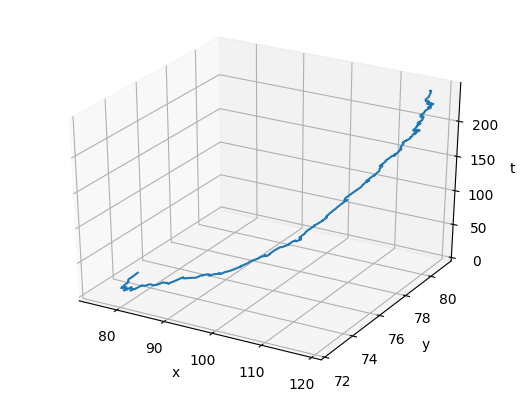
\includegraphics[width=\textwidth]{plots/small/H-GPOMDP-mu.png}
    \end{minipage}
    \vspace{0.5cm}
    \begin{minipage}{0.44\textwidth}
    	\setlength\figureheight{5cm}  
		\setlength\figurewidth{5cm}
		% This file was created by matplotlib2tikz v0.6.16.
\begin{tikzpicture}

\begin{axis}[
xlabel={x},
ylabel={y},
xmin=-50, xmax=200,
ymin=-50, ymax=200,
width=\figurewidth,
height=\figureheight,
tick align=outside,
tick pos=left,
x grid style={white!69.01960784313725!black},
y grid style={white!69.01960784313725!black}
]
\draw[draw=green!50.0!black,fill opacity=0] (axis cs:75.1317003831378,74.6768050837108) ellipse (79.9353395250666 and 79.9382234702847);
\draw[draw=blue,fill opacity=0] (axis cs:110.103388580383,78.5924390364371) ellipse (26.7223871913147 and 35.8134359062225);
\draw[draw=red,fill opacity=0] (axis cs:118.293361504868,80.6952184954765) ellipse (21.7729869463623 and 28.8294594115844);
\addplot [semithick, black, forget plot]
table {%
100 120
120 100
};
\end{axis}

\end{tikzpicture}
    \end{minipage}
    \caption[H-GPOMDP mean value and variance in small environment]{H-GPOMDOP. Left: Mean parameters of the high level policy parameters. Right: The areas in which the $95\%$ of the samples of the high level policy parameters fall into}
    \label{fig:small_h_gpomdp_mu_sigma}
\end{figure}
 
\begin{figure}[t!]
	\centering
    \begin{minipage}{0.55\textwidth}
        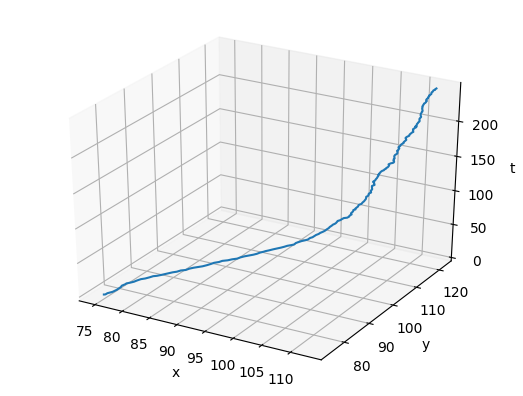
\includegraphics[width=\textwidth]{plots/small/H-PGPE-mu.png}
    \end{minipage}
    \begin{minipage}{0.44\textwidth}
    	\setlength\figureheight{5cm}  
		\setlength\figurewidth{5cm}
		% This file was created by matplotlib2tikz v0.6.16.
\begin{tikzpicture}

\begin{axis}[
xlabel={x},
ylabel={y},
xmin=-50, xmax=200,
ymin=-50, ymax=200,
width=\figurewidth,
height=\figureheight,
tick align=outside,
tick pos=left,
x grid style={white!69.01960784313725!black},
y grid style={white!69.01960784313725!black}
]
\draw[draw=green!50.0!black,fill opacity=0] (axis cs:74.7982194089664,74.5569367094516) ellipse (80.6292347223315 and 78.7779360974279);
\draw[draw=blue,fill opacity=0] (axis cs:105.612897286281,113.672809240917) ellipse (0.229782572592321 and 0.869859091279909);
\draw[draw=red,fill opacity=0] (axis cs:112.53500155361,121.909235094283) ellipse (-0.404669091261131 and -0.00279399170910306);
\addplot [semithick, black, forget plot]
table {%
100 120
120 100
};
\end{axis}

\end{tikzpicture}	
    \end{minipage}
    \caption[H-PGPE mean value and variance in small environment]{H-PGPE. Left: Mean parameters of the high level policy parameters. Right: The areas in which the $95\%$ of the samples of the high level policy parameters fall into}    
    \label{fig:small_h_pgpe_mu_sigma}
\end{figure}


\begin{figure}[t!]
	\centering
    \begin{minipage}{0.55\textwidth}
    	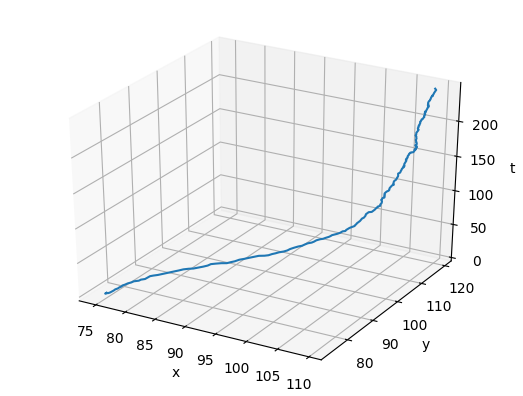
\includegraphics[width=\textwidth]{plots/small/H-PI-mu.png}
    \end{minipage}
    \begin{minipage}{0.44\textwidth}
    	\setlength\figureheight{5cm}  
		\setlength\figurewidth{5cm}
		% This file was created by matplotlib2tikz v0.6.16.
\begin{tikzpicture}

\begin{axis}[
xlabel={x},
ylabel={y},
xmin=-100, xmax=1100,
ymin=-100, ymax=1100,
width=\figurewidth,
height=\figureheight,
tick align=outside,
tick pos=left,
x grid style={white!69.01960784313725!black},
y grid style={white!69.01960784313725!black}
]
\draw[draw=green!50.0!black,fill opacity=0] (axis cs:497.976342114061,498.097206365816) ellipse (506.691499050605 and 507.762144923761);
\draw[draw=blue,fill opacity=0] (axis cs:396.384843374967,397.48448745119) ellipse (3.09446449865456 and 35.1597278943194);
\draw[draw=red,fill opacity=0] (axis cs:401.992682107541,399.80588469616) ellipse (1.14743217377442 and -0.869861990634435);
\addplot [semithick, black, forget plot]
table {%
350 400
450 400
};
\end{axis}

\end{tikzpicture}
    \end{minipage}
    \caption[H-PI mean value and variance in small environment]{H-PI. Left: Mean parameters of the high level policy parameters. Right: The areas in which the $95\%$ of the samples of the high level policy parameters fall into}
    \label{fig:small_h_pi_mu_sigma}
    
\end{figure}

\clearpage

\section{Results in Regular Domain}

The task in the regular ship steering domain possibly is too complex for the flat algorithms due to the larger state-space and random initialization of the ship position. Scaling the discretization from the small to the big environment makes the policy intractable. Therefore, experiments are conducted only with hierarchical algorithms that had a good performance in the small domain: H-PGPE and H-PI. 

The high level controllers use the GPOMDP algorithm to learn a multivariate Gaussian policy with diagonal standard deviation. Policy distribution mean is initialized in the middle of the map, that is $(500, 500)$. The variance of the two dimensions is 255. The algorithm fits every 40 episodes with an adaptive learning rate of 50. Horizon is 100 steps for both the low level and the high level algorithms.

A deterministic policy is constructed by using the absolute values of  weights, that is,  $\pi(x) = \left|\omega\right|x$ for the low level policies. PGPE algorithm learns the distribution over the weights that is initialized with zero mean and $10^{-3}$ variance. The algorithm fits every 10 episodes of the low level controller with an adaptive learning rate of $5\times10{-4}$. The action taken by the low level is a proportional control action for H-PGPE and proportional-integral for H-PI. 

The learning curves of the algorithms are given in Figure~\ref{fig:big_hier_J}. The values are computed with the mean of the objective function for every epoch, averaged for 100 experiments for each algorithm. Curves are slightly less steep than the ones of the smaller domain. This is because the regular domain task is harder. Figure~\ref{fig:big_hier_L} shows the average episode lengths for each epoch, for both algorithms. In the first epochs, low level learns to stay in the map and to follow the referenced angle. Once the high level algorithm detects the gate position, episodes become much shorter, to approximate the shortest path. 

\begin{figure}[t]
	\centering
    \setlength\figureheight{6cm}  
	\setlength\figurewidth{\textwidth}
	% This file was created by matplotlib2tikz v0.6.16.
\begin{tikzpicture}

\definecolor{color0}{rgb}{1,0.498039215686275,0.0549019607843137}

\begin{axis}[
xlabel={epoch},
ylabel={J},
xmin=-1.25, xmax=26.25,
ymin=-99.6868135838367, ymax=-86.1646488743638,
width=\figurewidth,
height=\figureheight,
tick align=outside,
tick pos=left,
ytick distance=2,
x grid style={white!69.01960784313725!black},
y grid style={white!69.01960784313725!black},
legend style={at={(0.03,0.97)}, anchor=north west, draw=white!80.0!black, font=\footnotesize},
legend cell align={left},
legend entries={{H-PGPE},{H-PI}}
]
\addlegendimage{no markers, blue}
\addlegendimage{no markers, color0}
\path [draw=blue, semithick] (axis cs:0,-98.6186432917592)
--(axis cs:0,-99.0721697334062);

\path [draw=blue, semithick] (axis cs:1,-97.3191400856202)
--(axis cs:1,-97.8178021915616);

\path [draw=blue, semithick] (axis cs:2,-97.3278734543125)
--(axis cs:2,-97.8491522869482);

\path [draw=blue, semithick] (axis cs:3,-96.4883726412631)
--(axis cs:3,-97.0522423665752);

\path [draw=blue, semithick] (axis cs:4,-95.3321362008732)
--(axis cs:4,-95.9618640658969);

\path [draw=blue, semithick] (axis cs:5,-93.2854433247004)
--(axis cs:5,-94.043623644619);

\path [draw=blue, semithick] (axis cs:6,-92.0833272273029)
--(axis cs:6,-93.0380850103506);

\path [draw=blue, semithick] (axis cs:7,-91.7688697330869)
--(axis cs:7,-92.640125764855);

\path [draw=blue, semithick] (axis cs:8,-91.4295546914821)
--(axis cs:8,-92.3550538777955);

\path [draw=blue, semithick] (axis cs:9,-90.1366372529003)
--(axis cs:9,-91.1408314789972);

\path [draw=blue, semithick] (axis cs:10,-89.3819097193017)
--(axis cs:10,-90.4569828250573);

\path [draw=blue, semithick] (axis cs:11,-88.6623202015229)
--(axis cs:11,-89.7871428591142);

\path [draw=blue, semithick] (axis cs:12,-88.2028771930043)
--(axis cs:12,-89.2885220246916);

\path [draw=blue, semithick] (axis cs:13,-88.0382573414197)
--(axis cs:13,-88.958562559077);

\path [draw=blue, semithick] (axis cs:14,-87.8354842344783)
--(axis cs:14,-88.7056492880469);

\path [draw=blue, semithick] (axis cs:15,-87.6855425682927)
--(axis cs:15,-88.5232913132147);

\path [draw=blue, semithick] (axis cs:16,-87.4473870237435)
--(axis cs:16,-88.2740763683597);

\path [draw=blue, semithick] (axis cs:17,-87.2568090777906)
--(axis cs:17,-88.0484866995881);

\path [draw=blue, semithick] (axis cs:18,-86.7792927247944)
--(axis cs:18,-87.7952475818047);

\path [draw=blue, semithick] (axis cs:19,-87.5104602783067)
--(axis cs:19,-88.288098992873);

\path [draw=blue, semithick] (axis cs:20,-87.1507000685934)
--(axis cs:20,-87.8272381042379);

\path [draw=blue, semithick] (axis cs:21,-86.8388083556658)
--(axis cs:21,-87.6314974459656);

\path [draw=blue, semithick] (axis cs:22,-87.0965359404103)
--(axis cs:22,-87.9233301161857);

\path [draw=blue, semithick] (axis cs:23,-87.0477044536614)
--(axis cs:23,-87.97837387626);

\path [draw=blue, semithick] (axis cs:24,-87.194786281133)
--(axis cs:24,-87.9462999653316);

\path [draw=blue, semithick] (axis cs:25,-87.2897392480625)
--(axis cs:25,-88.1143129161197);

\path [draw=color0, semithick] (axis cs:0,-98.5796385537277)
--(axis cs:0,-99.0309306475881);

\path [draw=color0, semithick] (axis cs:1,-97.5716316566127)
--(axis cs:1,-97.9918288268185);

\path [draw=color0, semithick] (axis cs:2,-97.0669784243078)
--(axis cs:2,-97.501113678087);

\path [draw=color0, semithick] (axis cs:3,-96.2342627825226)
--(axis cs:3,-96.7869267961619);

\path [draw=color0, semithick] (axis cs:4,-95.0329235446257)
--(axis cs:4,-95.7222100807895);

\path [draw=color0, semithick] (axis cs:5,-93.0937192877062)
--(axis cs:5,-93.8776043635349);

\path [draw=color0, semithick] (axis cs:6,-92.3350837476444)
--(axis cs:6,-93.0417769459607);

\path [draw=color0, semithick] (axis cs:7,-91.4788770484909)
--(axis cs:7,-92.3417237709249);

\path [draw=color0, semithick] (axis cs:8,-91.1310097701006)
--(axis cs:8,-92.047568338441);

\path [draw=color0, semithick] (axis cs:9,-90.4633856769803)
--(axis cs:9,-91.4919649627105);

\path [draw=color0, semithick] (axis cs:10,-89.4641388867949)
--(axis cs:10,-90.4410040316289);

\path [draw=color0, semithick] (axis cs:11,-88.7338270291225)
--(axis cs:11,-89.8049259445917);

\path [draw=color0, semithick] (axis cs:12,-88.072036361087)
--(axis cs:12,-89.075977943898);

\path [draw=color0, semithick] (axis cs:13,-88.0334231036403)
--(axis cs:13,-88.9630553438613);

\path [draw=color0, semithick] (axis cs:14,-87.5037462720889)
--(axis cs:14,-88.4244122807454);

\path [draw=color0, semithick] (axis cs:15,-87.6603391279723)
--(axis cs:15,-88.4998572973396);

\path [draw=color0, semithick] (axis cs:16,-87.3362260245575)
--(axis cs:16,-88.0921312903672);

\path [draw=color0, semithick] (axis cs:17,-87.2567126703445)
--(axis cs:17,-88.0716591757684);

\path [draw=color0, semithick] (axis cs:18,-87.1310731076264)
--(axis cs:18,-88.0129853278574);

\path [draw=color0, semithick] (axis cs:19,-86.960662621279)
--(axis cs:19,-87.7342131976424);

\path [draw=color0, semithick] (axis cs:20,-87.4994605608238)
--(axis cs:20,-88.2187986048138);

\path [draw=color0, semithick] (axis cs:21,-86.9885281246732)
--(axis cs:21,-87.8190471228839);

\path [draw=color0, semithick] (axis cs:22,-87.1373384630533)
--(axis cs:22,-87.8540316644523);

\path [draw=color0, semithick] (axis cs:23,-87.320752285901)
--(axis cs:23,-88.0645632405074);

\path [draw=color0, semithick] (axis cs:24,-86.9449738682615)
--(axis cs:24,-87.8696912413971);

\path [draw=color0, semithick] (axis cs:25,-87.3435372012375)
--(axis cs:25,-88.1321930489828);

\addplot [semithick, blue, forget plot]
table {%
0 -98.8454065125827
1 -97.5684711385909
2 -97.5885128706303
3 -96.7703075039191
4 -95.6470001333851
5 -93.6645334846597
6 -92.5607061188267
7 -92.2044977489709
8 -91.8923042846388
9 -90.6387343659487
10 -89.9194462721795
11 -89.2247315303186
12 -88.745699608848
13 -88.4984099502484
14 -88.2705667612626
15 -88.1044169407537
16 -87.8607316960516
17 -87.6526478886894
18 -87.2872701532995
19 -87.8992796355898
20 -87.4889690864157
21 -87.2351529008157
22 -87.509933028298
23 -87.5130391649607
24 -87.5705431232323
25 -87.7020260820911
};
\addplot [semithick, color0, forget plot]
table {%
0 -98.8052846006579
1 -97.7817302417156
2 -97.2840460511974
3 -96.5105947893422
4 -95.3775668127076
5 -93.4856618256205
6 -92.6884303468026
7 -91.9103004097079
8 -91.5892890542708
9 -90.9776753198454
10 -89.9525714592119
11 -89.2693764868571
12 -88.5740071524925
13 -88.4982392237508
14 -87.9640792764171
15 -88.0800982126559
16 -87.7141786574624
17 -87.6641859230565
18 -87.5720292177419
19 -87.3474379094607
20 -87.8591295828188
21 -87.4037876237786
22 -87.4956850637528
23 -87.6926577632042
24 -87.4073325548293
25 -87.7378651251101
};
\end{axis}

\end{tikzpicture}
    \caption[J comparison, regular environment]{Average of objective function of the hierarchical algorithms at every epoch}
    \label{fig:big_hier_J}
\end{figure}
\begin{figure}[t]
    \setlength\figureheight{6cm}  
	\setlength\figurewidth{\textwidth}
	% This file was created by matplotlib2tikz v0.6.16.
\begin{tikzpicture}

\definecolor{color0}{rgb}{1,0.498039215686275,0.0549019607843137}
\definecolor{color1}{rgb}{0.580392156862745,0.403921568627451,0.741176470588235}

\begin{axis}[
xlabel={epoch},
ylabel={episode length},
xmin=-1.25, xmax=26.25,
ymin=-34.915452394257, ymax=1141.7474948898,
width=\figurewidth,
height=\figureheight,
tick align=outside,
tick pos=left,
x grid style={white!69.01960784313725!black},
y grid style={white!69.01960784313725!black}
]
\path [draw=blue, semithick] (axis cs:0,81.0911760668363)
--(axis cs:0,79.7708239331638);

\path [draw=blue, semithick] (axis cs:1,489.404089545043)
--(axis cs:1,426.197910454957);

\path [draw=blue, semithick] (axis cs:2,1088.2628154678)
--(axis cs:2,883.186184532202);

\path [draw=blue, semithick] (axis cs:3,902.729243554014)
--(axis cs:3,668.031756445986);

\path [draw=blue, semithick] (axis cs:4,538.649445355297)
--(axis cs:4,388.479554644704);

\path [draw=blue, semithick] (axis cs:5,360.585648488226)
--(axis cs:5,256.607351511774);

\path [draw=blue, semithick] (axis cs:6,206.965204754822)
--(axis cs:6,168.017795245178);

\path [draw=blue, semithick] (axis cs:7,169.231441872846)
--(axis cs:7,133.929558127155);

\path [draw=blue, semithick] (axis cs:8,133.475028224666)
--(axis cs:8,114.202971775334);

\path [draw=blue, semithick] (axis cs:9,120.197500073287)
--(axis cs:9,102.460499926713);

\path [draw=blue, semithick] (axis cs:10,104.727491148319)
--(axis cs:10,94.9935088516812);

\path [draw=blue, semithick] (axis cs:11,108.924620800781)
--(axis cs:11,95.2993791992188);

\path [draw=blue, semithick] (axis cs:12,104.255991538558)
--(axis cs:12,93.2330084614424);

\path [draw=blue, semithick] (axis cs:13,98.0292641895068)
--(axis cs:13,92.0547358104933);

\path [draw=blue, semithick] (axis cs:14,98.8711748590563)
--(axis cs:14,90.1158251409437);

\path [draw=blue, semithick] (axis cs:15,93.3654467977495)
--(axis cs:15,89.5665532022504);

\path [draw=blue, semithick] (axis cs:16,97.5575558096076)
--(axis cs:16,90.2624441903923);

\path [draw=blue, semithick] (axis cs:17,97.9323236248251)
--(axis cs:17,91.0486763751749);

\path [draw=blue, semithick] (axis cs:18,95.5247837818183)
--(axis cs:18,90.2502162181817);

\path [draw=blue, semithick] (axis cs:19,94.023289405138)
--(axis cs:19,89.856710594862);

\path [draw=blue, semithick] (axis cs:20,92.2067689802821)
--(axis cs:20,89.3982310197179);

\path [draw=blue, semithick] (axis cs:21,93.391101891151)
--(axis cs:21,89.895898108849);

\path [draw=blue, semithick] (axis cs:22,93.3524553428036)
--(axis cs:22,90.0975446571963);

\path [draw=blue, semithick] (axis cs:23,97.7341276584202)
--(axis cs:23,88.6568723415798);

\path [draw=blue, semithick] (axis cs:24,90.3209027734668)
--(axis cs:24,88.8900972265332);

\path [draw=blue, semithick] (axis cs:25,92.5221037823311)
--(axis cs:25,89.4808962176688);

\path [draw=color0, semithick] (axis cs:0,80.8898148348609)
--(axis cs:0,79.4681851651391);

\path [draw=color0, semithick] (axis cs:1,439.120094554962)
--(axis cs:1,377.640905445038);

\path [draw=color0, semithick] (axis cs:2,1032.95442974765)
--(axis cs:2,842.891570252345);

\path [draw=color0, semithick] (axis cs:3,856.783597826666)
--(axis cs:3,675.807402173334);

\path [draw=color0, semithick] (axis cs:4,591.144024461649)
--(axis cs:4,447.192975538351);

\path [draw=color0, semithick] (axis cs:5,320.693359972832)
--(axis cs:5,257.479640027168);

\path [draw=color0, semithick] (axis cs:6,210.400236336701)
--(axis cs:6,167.771763663299);

\path [draw=color0, semithick] (axis cs:7,151.610366773235)
--(axis cs:7,124.861633226765);

\path [draw=color0, semithick] (axis cs:8,127.940874876469)
--(axis cs:8,112.022125123531);

\path [draw=color0, semithick] (axis cs:9,118.527082951398)
--(axis cs:9,104.114917048602);

\path [draw=color0, semithick] (axis cs:10,105.946442170183)
--(axis cs:10,97.0455578298172);

\path [draw=color0, semithick] (axis cs:11,105.632499394661)
--(axis cs:11,93.9745006053392);

\path [draw=color0, semithick] (axis cs:12,98.3736022287574)
--(axis cs:12,92.9923977712426);

\path [draw=color0, semithick] (axis cs:13,95.7685447996079)
--(axis cs:13,91.4294552003921);

\path [draw=color0, semithick] (axis cs:14,96.2767949771307)
--(axis cs:14,89.8092050228693);

\path [draw=color0, semithick] (axis cs:15,92.2745034094563)
--(axis cs:15,89.8884965905437);

\path [draw=color0, semithick] (axis cs:16,93.3287433870181)
--(axis cs:16,90.1812566129819);

\path [draw=color0, semithick] (axis cs:17,91.8728528575949)
--(axis cs:17,89.3481471424052);

\path [draw=color0, semithick] (axis cs:18,93.264917045919)
--(axis cs:18,89.6680829540809);

\path [draw=color0, semithick] (axis cs:19,92.7231665552644)
--(axis cs:19,89.4238334447355);

\path [draw=color0, semithick] (axis cs:20,95.5063672858701)
--(axis cs:20,90.08563271413);

\path [draw=color0, semithick] (axis cs:21,91.2686813137062)
--(axis cs:21,89.0083186862937);

\path [draw=color0, semithick] (axis cs:22,90.8035134720861)
--(axis cs:22,88.650486527914);

\path [draw=color0, semithick] (axis cs:23,92.3091956446672)
--(axis cs:23,89.1378043553328);

\path [draw=color0, semithick] (axis cs:24,93.5936523439909)
--(axis cs:24,89.6223476560091);

\path [draw=color0, semithick] (axis cs:25,92.3530804421264)
--(axis cs:25,89.4229195578736);

\path [draw=color1, semithick] (axis cs:0,21.4947729722544)
--(axis cs:0,18.5692270277456);

\path [draw=color1, semithick] (axis cs:1,177.082150179711)
--(axis cs:1,110.338849820289);

\path [draw=color1, semithick] (axis cs:2,340.643305773912)
--(axis cs:2,183.941694226088);

\path [draw=color1, semithick] (axis cs:3,360.332570573641)
--(axis cs:3,215.438429426359);

\path [draw=color1, semithick] (axis cs:4,277.493936776158)
--(axis cs:4,168.064063223841);

\path [draw=color1, semithick] (axis cs:5,257.145558889606)
--(axis cs:5,152.756441110393);

\path [draw=color1, semithick] (axis cs:6,228.023642986969)
--(axis cs:6,109.413357013031);

\path [draw=color1, semithick] (axis cs:7,279.080792455482)
--(axis cs:7,74.3622075445179);

\path [draw=color1, semithick] (axis cs:8,251.4236248622)
--(axis cs:8,66.5243751377995);

\path [draw=color1, semithick] (axis cs:9,231.433418374939)
--(axis cs:9,39.5205816250608);

\path [draw=color1, semithick] (axis cs:10,200.793117170882)
--(axis cs:10,59.4268828291176);

\path [draw=color1, semithick] (axis cs:11,173.736892736264)
--(axis cs:11,75.6181072637357);

\path [draw=color1, semithick] (axis cs:12,120.422034306393)
--(axis cs:12,64.6239656936068);

\path [draw=color1, semithick] (axis cs:13,154.479879676207)
--(axis cs:13,61.065120323793);

\path [draw=color1, semithick] (axis cs:14,207.460464821122)
--(axis cs:14,33.8015351788782);

\path [draw=color1, semithick] (axis cs:15,206.070374646037)
--(axis cs:15,35.3876253539627);

\path [draw=color1, semithick] (axis cs:16,215.924292317934)
--(axis cs:16,28.9867076820658);

\path [draw=color1, semithick] (axis cs:17,98.0872237981273)
--(axis cs:17,52.4477762018727);

\path [draw=color1, semithick] (axis cs:18,87.9319820355879)
--(axis cs:18,58.4950179644121);

\path [draw=color1, semithick] (axis cs:19,79.9470258352977)
--(axis cs:19,57.9949741647023);

\path [draw=color1, semithick] (axis cs:20,177.12603638901)
--(axis cs:20,26.7319636109902);

\path [draw=color1, semithick] (axis cs:21,127.835610127343)
--(axis cs:21,41.2623898726565);

\path [draw=color1, semithick] (axis cs:22,93.3663605082555)
--(axis cs:22,57.6176394917445);

\path [draw=color1, semithick] (axis cs:23,80.6185662904916)
--(axis cs:23,59.8684337095084);

\path [draw=color1, semithick] (axis cs:24,79.6719092223636)
--(axis cs:24,60.0990907776364);

\path [draw=color1, semithick] (axis cs:25,81.8456657834132)
--(axis cs:25,61.6783342165868);

\addplot [semithick, blue, forget plot]
table {%
0 80.4310000000001
1 457.801
2 985.7245
3 785.3805
4 463.5645
5 308.5965
6 187.4915
7 151.5805
8 123.839
9 111.329
10 99.8605
11 102.112
12 98.7445
13 95.042
14 94.4935
15 91.466
16 93.91
17 94.4905
18 92.8875
19 91.94
20 90.8025
21 91.6435
22 91.725
23 93.1955
24 89.6055
25 91.0015
};
\addplot [semithick, color0, forget plot]
table {%
0 80.179
1 408.3805
2 937.923
3 766.2955
4 519.1685
5 289.0865
6 189.086
7 138.236
8 119.9815
9 111.321
10 101.496
11 99.8035
12 95.683
13 93.599
14 93.043
15 91.0815
16 91.755
17 90.6105
18 91.4665
19 91.0735
20 92.796
21 90.1385
22 89.727
23 90.7235
24 91.608
25 90.888
};
\addplot [semithick, color1, forget plot]
table {%
0 20.032
1 143.7105
2 262.2925
3 287.8855
4 222.779
5 204.951
6 168.7185
7 176.7215
8 158.974
9 135.477
10 130.11
11 124.6775
12 92.523
13 107.7725
14 120.631
15 120.729
16 122.4555
17 75.2675
18 73.2135
19 68.971
20 101.929
21 84.549
22 75.492
23 70.2435
24 69.8855
25 71.762
};
\end{axis}

\end{tikzpicture}
    \caption[Episode length comparison, regular environment]{Average episode lengths of hierarchical algorithms at every epoch}
    \label{fig:big_hier_L}
\end{figure}

\clearpage

Figure~\ref{fig:big_traj_h_pgpe} depicts the trajectories of the last 5 episodes of the epochs 0, 3, 12 and 24 for the H-PGPE algorithm and Figure~\ref{fig:big_traj_h_pi} shows that of the H-PI algorithm. The trajectories start at random points as the high level task requires. In both figures we observe a stroll around the gate at the last steps. This is because the ship starts at random points and the gate is in the middle of the map. These characteristics of the regular domain eliminate the possibility of placing the reference position behind the gate. Moreover, when the ship is almost reaching the gate, low level policy performance is lousy. We observe a negative peak in the low level intrinsic reward as the angle difference jumps from 0 to $\pi$ while the ship trespass the reference point.


\figuretraj{big}{H-PGPE}{H-PGPE trajectories, regular environment}{hierarchical algorithm with PGPE in the low level, last 5 trajectories of the epochs}{fig:big_traj_h_pgpe}
\figuretraj{big}{H-PI}{H-PI trajectories, regular environment}{hierarchical algorithm with PGPE in the low level, with integral action, last 5 trajectories of the epochs}{fig:big_traj_h_pi}

 
 The average of the parameters of the hierarchical algorithm with PGPE in the low level (H-PGPE) is shown in Figure~\ref{fig:big_h_pgpe_mu_sigma}. Figure~\ref{fig:big_h_pi_mu_sigma} demonstrates the same observations for hierarchical algorithm with PGPE learning a policy with integral action in the low level (H-PI). We observe that both algorithms are able to identify the gate position quite fast, almost as fast as they identified the gate in the small domain. The fast convergence is explained by the fact that the position of the gate is near to the middle of the map and the initial distribution of the high level is centered in there. 

\begin{figure}[t]
	\centering
    \begin{minipage}{0.55\textwidth}
        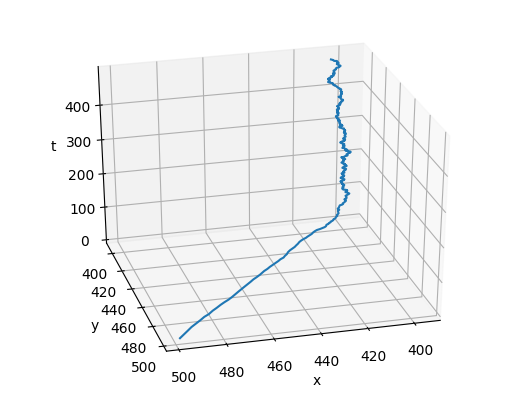
\includegraphics[width=\textwidth]{plots/big/H-PGPE-mu.png}
    \end{minipage}
    \begin{minipage}{0.44\textwidth}
    	\setlength\figureheight{5cm}  
		\setlength\figurewidth{5cm}
		% This file was created by matplotlib2tikz v0.6.16.
\begin{tikzpicture}

\begin{axis}[
xlabel={x},
ylabel={y},
xmin=-50, xmax=200,
ymin=-50, ymax=200,
width=\figurewidth,
height=\figureheight,
tick align=outside,
tick pos=left,
x grid style={white!69.01960784313725!black},
y grid style={white!69.01960784313725!black}
]
\draw[draw=green!50.0!black,fill opacity=0] (axis cs:74.7982194089664,74.5569367094516) ellipse (80.6292347223315 and 78.7779360974279);
\draw[draw=blue,fill opacity=0] (axis cs:105.612897286281,113.672809240917) ellipse (0.229782572592321 and 0.869859091279909);
\draw[draw=red,fill opacity=0] (axis cs:112.53500155361,121.909235094283) ellipse (-0.404669091261131 and -0.00279399170910306);
\addplot [semithick, black, forget plot]
table {%
100 120
120 100
};
\end{axis}

\end{tikzpicture}
    \end{minipage}
    \caption[H-PGPE mean value and variance in regular environment]{H-PGPE in regular domain. Left: Mean parameters of the high level policy parameters. Right: The areas in which the $95\%$ of the samples of the high level policy parameters fall into}
    \label{fig:big_h_pgpe_mu_sigma}
\end{figure}


\begin{figure}[t]
	\centering
    \begin{minipage}{0.55\textwidth}
    	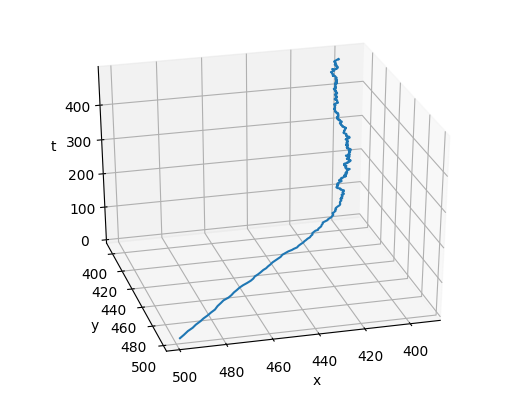
\includegraphics[width=\textwidth]{plots/big/H-PI-mu.png}
    \end{minipage}
    \begin{minipage}{0.44\textwidth}
    	\setlength\figureheight{5cm}  
		\setlength\figurewidth{5cm}
		% This file was created by matplotlib2tikz v0.6.16.
\begin{tikzpicture}

\begin{axis}[
xlabel={x},
ylabel={y},
xmin=-100, xmax=1100,
ymin=-100, ymax=1100,
width=\figurewidth,
height=\figureheight,
tick align=outside,
tick pos=left,
x grid style={white!69.01960784313725!black},
y grid style={white!69.01960784313725!black}
]
\draw[draw=green!50.0!black,fill opacity=0] (axis cs:497.976342114061,498.097206365816) ellipse (506.691499050605 and 507.762144923761);
\draw[draw=blue,fill opacity=0] (axis cs:396.384843374967,397.48448745119) ellipse (3.09446449865456 and 35.1597278943194);
\draw[draw=red,fill opacity=0] (axis cs:401.992682107541,399.80588469616) ellipse (1.14743217377442 and -0.869861990634435);
\addplot [semithick, black, forget plot]
table {%
350 400
450 400
};
\end{axis}

\end{tikzpicture}
    \end{minipage}
    \caption[H-PI mean value and variance in regular environment]{H-PI in regular domain. Left: Mean parameters of the high level policy parameters. Right: The areas in which the $95\%$ of the samples of the high level policy parameters fall into}
    \label{fig:big_h_pi_mu_sigma}
\end{figure}



\chapter{Conclusions and Future works}
\label{conclusions}
\thispagestyle{empty}

\begin{quotation}
{\footnotesize
\noindent{\emph{``Teacher Rick: Tomorrow you will be transferred to your new Ricks. Hopefully they will be your last. Yes, Slow Ri-- Tall Morty? \\
Tall Morty (Slow Rick): Di-Did I gragitate this time yet? \\
Teacher Rick: Anything’s possible, Tall Morty. Ugh… ''}}
\begin{flushright}
Rick and Morty (Season 3, Episode 7)
\end{flushright}
}
\end{quotation}



\vspace{0.5cm}

We developed a novel framework to design hierarchical structure in reinforcement learning that exploits the design tool of control theory: the block diagram. To achieve this, the block diagram is adapted to the context of hierarchical reinforcement learning. Our framework describes a computational graph that contains blocks and connections. Unlike the block diagram of control theory, in our approach blocks and the interconnections are of various nature. The type of connection depends on the use of the signal it carries, whereas the type of the block depends on the subsystem it represents. 

By running the computational graph, the hierarchical agent can interact with the environment and update all levels of its hierarchy. Similarly to the block diagram of the control theory, this framework can be applied to implement different types of hierarchical topologies. Therefore, the designer is free to implement his/her own hierarchical structure. Combining the strengths of both fields, we filled up a gap between control theory and machine learning.

Hierarchical approaches simplify the tasks of designing a policy and possibly adding prior knowledge: with our framework, we can exploit the existing hierarchical control structures and initial parameters for the well-known problems of control theory. Adapting a control theoretical perspective, policies are often simpler to interpret and with fewer parameters, without losing representation power. In control theoretic approaches, typically a human operator is needed to close the control loop for high level logic. With our framework we can assign the task of the human operator to a suitable learning agent. 
  
These advantages makes our framework suitable for complex robotics tasks, even with continuous action-spaces and high state-action dimensionality because the problem can be easily decomposed into different abstraction layers. The lower levels can control directly the actuators of the robot whereas the higher levels can focus on the more generic and complex tasks. 

Existing methods to introduce hierarchy to reinforcement learning are based on the idea of partial policies with well defined termination conditions. MAXQ uses stack discipline to execute the hierarchical policy. Options framework adds the subtasks to the available action set. HAMs constrain the low level policy. Despite the fact that we can implement partial policies, we should take an action also in the last step of the low level episode. This is due to the fact that, differently from the other HRL approaches, our computational graph executes continuously, that is, blocks operate sequentially and only in one direction. An outcome of this feature is that the agents in the lower levels of the hierarchy must take an action even in the last steps of their episodes. It is not possible to go back to the higher level controller during the cycle. Another cycle is needed to reset and start a new episode for the low level controller that has its episode finished. This is the fundamental difference between our approach and the state of the art. A subtask cannot exist by itself but is always part of the complete system.

Designing hierarchical algorithms is not trivial due to the interaction between the layers. Typically, the algorithms in different layers are not aware of each other performance. They do not know about each other tasks. This causes the agents to interpret the outcomes in a wrong way. For instance, if the outcome of the environment is bad after the execution of an action drawn by an agent, the agent that receives the bad reward will assume the poor performance is due to its choice, and updates its quality to avoid such policy, even when it is not the case. In addition, since the agents observe the environment only partially, and it may change its dynamics due to the actions of other layers, their perception of the environment is non-stationary. This problem is more clearly seen in our framework. Blocks observe the environment only through their connections. This means that their observation over the graph is only partial and, as it changes in time, it is non-stationary. This behavior can be clearly identified in the ship steering environment: when the high level policy has not yet identified the gate position, low level agent learns a policy stating that it should not to follow the reference of the high level agent, and learning becomes unstable. To avoid the instability of the low level controller, we used a deterministic policy that guarantees the stability criterion. 

We used this framework as a tool to build a hierarchical reinforcement learning solution for the ship steering problem that has continuous state-action space. Ship steering task is suitable for hierarchical decomposition and our control theoretic decomposition approach is easily adopted. The higher level subtask is defined as estimating the reference points in the map for the low level to follow and pass through a gate that is in an unknown fixed position. The low level subtask is to manipulate the rudder to decrease the error between the reference angle and the actual angle. A function block is added between these controllers to convert the reference position output of the high level controller to angle error input of the low level controller. Flat REPS and RWR algorithms learn faster than the hierarchical algorithms in the small domain. However, they suffer from premature convergence. Our frameworks performance is more stable and reliable compared to flat RWR and REPS and much faster than the flat PG algorithms. In the regular domain, learning curve is steeper when the learning algorithm of the low level controller is a black box optimization method. Also in the regular domain, the hierarchical algorithms built with our framework showed good performance in terms of learning speed and stability.

The task decomposition of the ship steering problem has a cascaded control structure as in DC motor control example. The framework supports building more complex hierarchical control systems such as those typical for hybrid systems. This can be achieved with selector blocks. Selector blocks implement the mode switching behavior in our framework. They contain block lists and activate one list at each cycle. 

The proposed framework should be tested in more challenging environments and with more complex learning algorithms. Learning speed can be improved using off policy learning methods, exploiting the performance of the active controller to update the policy also of inactive controllers. This would result in more algorithms learning in parallel, similar to intra-option learning.

Another important issue to analyze is the fact that each controller see the rest of the system as a partially observable and non-stationary environment. Both distributed and global learning algorithm should be considered to face this issue and speed up learning. 

% 1) Brief summary of what we did, explain how we bring the gap between Control theory and ML
% 2) Explain why a hierarchical policy is better than a flat one, advantages and disadvantages
% 3) talk about the difference with the options, maxq and other frameworks. Talk about the termination condition of the blocks, and the fact that we must take a last action
% 4) Talk about the issue of the approach: each controller see the rest of the system as a partially observable nonstationary environment
% 5) talk about the good results achieved in the ship steering environment
% 6) Talk briefly that we can add support for the hybrid system control stuff, with the selector block.
% 7) Future works: explain that the approach need to be tested in more challenging environments and more complex learning: e.g. learning off policy using a mux block (that means, more algorithm learning in parallel, intra policy learning). Say that the issue of nostationarity and partial observability should be taken seriosly in consideration


 


\cleardoublepage
% ---- Bibliography ----
\addcontentsline{toc}{chapter}{Bibliografy}
\bibliographystyle{plain}
\pagenumbering{Roman}
\bibliography{hierarchical}

% \appendix

% \pagestyle{fancy} 
% \fancyfoot{}                                               
% \renewcommand{\chaptermark}[1]{\markboth{\appendixname\ \thechapter.\ #1}{}} 
% \renewcommand{\sectionmark}[1]{\markright{\thesection.\ #1}}         
% \fancyhead[LE,RO]{\bfseries\thepage}    
                                        
% \fancyhead[RE]{\bfseries\leftmark}    
% \fancyhead[LO]{\bfseries\rightmark}     
% \renewcommand{\headrulewidth}{0.3pt} 

%\include{appendiceA}
%\include{appendiceB}
%\include{appendiceC}
%\include{appendiceD}
%\include{appendiceE}
%\include{appendiceF}

\end{document}





